% !TeX spellcheck = pl_PL
\documentclass[a4paper,twoside]{article}
\usepackage{polski}
\usepackage[utf8]{inputenc}
\usepackage{graphicx}
\usepackage{amsmath}

\usepackage[unicode, bookmarks=true]{hyperref} %do zakładek
\usepackage{tabto} % do tabulacji
\NumTabs{6} % globalne ustawienie wielkosci tabulacji
\usepackage{array}
\usepackage{multirow}
\usepackage{array}
\usepackage{dcolumn}
\usepackage{bigstrut}
\usepackage{color}
\usepackage[usenames,dvipsnames]{xcolor}
\usepackage{pdfpages}


\setlength{\textheight}{24cm}
\setlength{\textwidth}{15.92cm}
\setlength{\footskip}{10mm}
\setlength{\oddsidemargin}{0mm}
\setlength{\evensidemargin}{0mm}
\setlength{\topmargin}{0mm}
\setlength{\headsep}{5mm}

\newcolumntype{M}[1]{>{\centering\arraybackslash}m{#1}}
\newcolumntype{N}{@{}m{0pt}@{}}

\graphicspath{ {./images/} }

\definecolor{nie}{RGB}{178,34,34}
\definecolor{tak}{RGB}{0,120,0}

% === Reset inkrementacji sekcji przy nowym parcie === %
\usepackage{titlesec}

\makeatletter
\@addtoreset{section}{part}
\makeatother
\titleformat{\part}[display]
{\normalfont\LARGE\bfseries\centering}{}{0pt}{}


\begin{document}
\bibliographystyle{plain}



\begin{titlepage}
\title{\huge Interfejsy w Systemach Komputerowych - ULTIMATE}
\author{\large SonMati \\ Ervelan \\ Doxus}
\maketitle
\end{titlepage}

%===============================================================================
%*** PYTANIA I ODPOWIEDZI ******************************************************
%===============================================================================
\part{Pytania i odpowiedzi}

\section{\textcolor{blue}{RS-232}}
\subsection*{Prawda/Fałsz}
\begin{itemize}
	\item \textcolor{nie}{RS-232 jest portem przeznaczonym do synchronicznej transmisji znakowej. Generator taktu odpowiedzialny za wyprowadzanie znaków typowo ustawiany jest na: 1200bd, 2400bd, 4800bd, 9600bd, 19200bd.} \\
	{\small \emph{RS-232 jest portem przeznaczonym do asynchronicznej transmisji znakowej. Da się sztucznie stworzyć synchroniczną transmisję.}}
	
	\item \textcolor{tak}{Linie kontrolne w interfejsie RS-232 to: DTR, DSR, RTS, CTS, RI, DCD. Pary DTR/DSR i RTS/CTS wykorzystywane są do realizacji handshake'u w połączeniach bezmodemowych.} \\ {\small \emph{Tak, te pary linii mogą być wykorzystywane do handshake podczas gdy RxD i TxD zajmują się przesyłem danych.}}
	
	\item \textcolor{nie}{Transakcja w systemie MODBUS składa się z zapytania (query) wysyłanego przez stację Slave i odpowiedzi odsyłanej przez stację Master.} \\
	{\small \emph {Jest odwrotnie - zapytanie wysyła Master, a odpowiedź odsyła Slave.}}
	
	\item \textcolor{nie}{W trybie transmisji ASCII znacznikiem początku ramki jest znak ':', a kooca ramki para znaków CR LF. W trybie transmisji RTU znacznikiem początku ramki jest znak 'Ctrl-A', a kooca para znaków CTRL-Y CTRL-Z.} \\
	{\small \emph{Zdanie jest poprawne dla ASCII. Dla RTU, znacznikiem początku i końca ramki jest przerwa o długości minimum 4T, gdzie T jest czasem trwania jednego znaku.}}
	
	\item \textcolor{nie}{Standard RS-232 transmituje znaki synchronicznie, bity w znakach [asynchronicznie]} \\
	{\small \emph{Ostatnie słowo ucięte, więc spekuluję że tak właśnie było napisane. To nieprawda, jest odwrotnie.}}
	
	\item \textcolor{tak}{Standard RS-422 pozwala na osiągnięcie szybkości 10MBodów na odległości 100m.} \\
	{\small \emph{IMO pozwala, na slajdzie 12 jest napisane że 10 Mbd przy zasięgu DO 100m - czyli 100m chyba też.}}
	
	\item \textcolor{tak}{Liniami kontrolnymi w RS-232 nie są linie TxD, RxD, SG.} \\
	{\small \emph{Owszem, TxD i RxD są liniami danych, a SG to po prostu masa.}}
	
	\item \textcolor{tak}{System MODBUS składa się z faz zapytania i odpowiedzi.} \\
	{\small \emph{Tak właśnie jest.}}
	
	\item {W systemie MODBUS}
	\begin{itemize}
		\item \textcolor{tak}{Obowiązuje master/slave.} \\
		{\small \emph{Pewnie, a w dodatku Slave'ów może być wielu.}}
		
		\item \textcolor{tak}{Prędkości transmisji wynoszą od 1200 do 19200bd.} \\
		{\small \emph{Jak najbardziej.}}
		
		\item \textcolor{tak}{Ramka w ASCII może mieć format 7N2 (lub np. 7E1, 7O1).} \\
		{\small \emph{Tak, patrz warstwa fizyczna MODBUS.}}
		
		\item \textcolor{tak}{Ramka w RTU może mieć format 8N2 *(lub np. 8E1, 8O1).} \\
		{\small \emph{Tak, patrz warstwa fizyczna MODBUS.}}
	\end{itemize} 
	
	
	\item \textcolor{tak}{W trybie transmisji RTU jest kontrola błędów CRC.} \\
	{\small \emph{Tak, jest elementem budowy ramki RTU.}}
	
	\item \textcolor{nie}{Bit kontrolny w RS-232 zależy od bitu danych i bitu stopu.} \\
	{\small \emph{Bit kontrolny słuzy do kontroli parzystości/nieparzystości, nie ma związku z bitem stopu.}}
	
	\item \textcolor{nie}{Za pomocą RS-232 możemy połączyć ze sobą 2 stacje DCE} \\
	{\small \emph{Połączyć możemy dwie stacje DTE, lub DTE z DCE. Dwie stacje DCE łączą się za pomocą łącza telefonicznego.}}
	
	\item \textcolor{tak}{W MODBUS kontrola błędów jest realizowana za pomocą LRC lub CRC.} \\
	{\small \emph{Tak, LRC wykorzystywane jest w trybie ASCII, CRC w trybie RTU.}}
	
	\item \textcolor{nie}{Do portu RS 485 można podłączyć tylko jedno urządzenie, ale za to obsługiwać go z dużo większą szybkością i na większą odległość niż jest to możliwe w przypadku interfejsu RS 232.} \\
	{\small \emph{Można podłączyć do 32 stacji.}}
	
	\item \textcolor{nie}{Format ramki w protokole Modbus jest następujący: znacznik początku ramki, adres urządzenia slave, adres mastera, pole danych, znacznik końca ramki.} \\
	{\small \emph{Opis nie pasuje ani do trybu ASCII, ani RTU}}
	
	\item \textcolor{nie}{RS 232 jest portem przeznaczonym dla asynchronicznej transmisji znakowej, realizowanej zazwyczaj w trybie dupleksowym, czyli dwukierunkowej transmisji niejednoczenej (naprzemiennej)} \\
	{\small \emph{Tryb dupleksowy jest równoczesny, to półdupleksowy jest niejednoczesny.}}
	
	\item \textcolor{tak}{W interfejsie RS 232 linie TxD i RxD służą do transmisji znaków, natomiast DTR, RTS to wyjścia kontrolne, a DSR, CTS, RI i DCD to wejścia kontrolne.} \\
	{\small \emph{Indeed}}
	
	\item \textcolor{tak}{Multipleksowanie urządzeń ze znakowym portem asynchronicznym pozwala na ich kontrolę poprzez jeden port RS-232.} \\
	{\small \emph{Żeby kontrolować kilka urządzeń z jednego portu potrzebny jest koncentrator. Jeśli "używanie koncentratora" równa się "multipleksowanie", to PRAWDA.}}
	
	\item \textcolor{tak}{Węzeł podrzędny w systemie MODBUS po wykryciu błędu w komunikacie wysyła potwierdzenie negatywne	do węzła nadrzędnego.} \\
	{\small \emph{W odpowiedzi pole to jest wykorzystywane do pozytywnego lub negatywnego potwierdzenia wykonania polecenia.}}
	
	\item \textcolor{tak}{Czy w trybie ASCII systemu MODBUS każdy bajt wysyłany jest jako znak z przedziału 0x00, 0xFF?} \\
	{\small \emph{Bajt dzielimy na 2 części i wysyłamy jako 2 znaki z przedziału 0-9 i Ah-Fh}}
		
	
\end{itemize}


\section{\textcolor{blue}{USB}}
\subsection*{Prawda/Fałsz}
\begin{itemize}
	
	\item \textcolor{tak}{Kontrola urządzenia USB odbywa się poprzez zapisy komunikatów do bufora o numerze 0 i odczycie informacji statusowych z bufora o numerze 0.} \\
	{\small \emph{Zgadza się.}}
	
	\item \textcolor{nie}{W przypadku błędu transmisji każda transakcja USB jest powtarzana, ponieważ niedopuszczalne jest przekazywanie danych przekłamanych.} \\
	{\small \emph{Transakcje izochroniczne nie są powtarzane w przypadku błędu transmisji.}}
	
	\item \textcolor{tak}{Hub nie dopuszcza ruchu full speed do portów, do których są podłączone urządzenia low speed.} \\
	{\small \emph{Tak, urządzenie lowspeed blokuje możliwość włączenia fullspeed na całym porcie.}}
	
	\item \textcolor{nie}{Reset portu USB polega na rekonfiguracji hosta, po której host zapisuje tablicę deskryptorów do urządzenia podłączonego do tego portu.} \\
	{\small \emph{Reset portu USB polega na rekonfiguracji urządzenia. W następującej procedurze enumeracji między innymi dochodzi do odczytu tablicy deskryptorów z urządzenia przez host.}}
	
	\item \textcolor{nie}{Typowa transakcja USB składa się z pakietów żądania i odpowiedzi, z których każdy potwierdzany jest osobnym potwierdzeniem.} \\
	{\small \emph{Typowa transakcja USB składa sie z pakietów token, data i handshake. Transakcje izochroniczne nie są potwierdzane.}}
	
	\item \textcolor{nie}{W systemie USB urządzenia zgłaszają żądania do hosta, który je kolejkuje i następnie obsługuje w kolejności pojawiania się zgłoszenia.} \\
	{\small \emph{Urządzenia nie zgłaszają żądania, tylko są odpytywane przez hosta. Host nie tworzy jednej kolejki, tylko w miarę możliwości stara się obsługiwać wszystkie urządzenia jednocześnie, równomiernie, zapobiegając zawłaszczeniu.}}
	
	\item \textcolor{nie}{W USB można połączyd kaskadowo do 5 hubów, korzystających z zasilania magistralowego} \\
	{\small \emph{Podłączyć je można tylko korzystając z zasilania zewnętrznego lub hybrydowego. Przy zasilaniu magistralowym zabraknie zasilania już na drugim hubie. Co więcej, należy mieć na uwadze maksymalne dopuszczalne opóźnienie sygnału, które przy przejściu przez 5 hubów jest osiągane - 350ns. Urządzenia podpięte do 5'tego huba mogą nie działać poprawnie.}}
	
	\item \textcolor{nie}{Mechanizm data toggle w USB służy do przywracania synchronizacji pomiędzy hostem i urządzeniem, utraconej na skutek wystąpienia błędów w pakietach danych.} \\
	{\small \emph{Mechanizm data toggle zabezpiecza przed utratą synchronizacji pomiędzy hostem i urządzeniem na skutek błędu w potwierdzeniu odsyłanym przez odbiorcę.}}
	
	\item \textcolor{tak}{Host kontroler USB komunikuje się z interfejsem magistrali USB urządzenia peryferyjnego za pomocą fizycznego kanału komunikacyjnego.} \\
	{\small \emph{Tak, używamy kabelka.}}
	
	\item \textcolor{nie}{Kamera internetowa może przesyłać obraz do komputera za pomocą transferu izochronicznego z szybkością LowSpeed w interfejsie USB.} \\
	{\small \emph{Z tabelki można wyczytać, że dla transferu izochronicznego nie można wykorzystać szybkości LowSpeed.}}
	
	\item \textcolor{tak}{Pakiety USB przesyłane z szybkością LowSpeed muszą byd poprzedzone pakietem preambuły} \\
	{\small \emph{Tak, jest on charakterystyczny dla pakietów przesyłanych z szybkością LowSpeed}}
	
	\item \textcolor{nie}{Urządzenie peryferyjne USB 2.0 może być podłączone do host kontrolera za pośrednictwem maksymalnie sześciu hubów.} \\
	{\small \emph{Aby spełnić normę (ograniczenie czasowe oczekiwania na odpowiedź), można podłączyd za pośrednictwem maksymalnie 5 hubów.}}
	
	\item \textcolor{nie}{Pole PID w pakiecie USB zabezpieczone jest 16-bitową sumą kontrolną CRC.} \\
	{\small \emph{Pole PID zabezpieczone jest 4-bitowym polem kontroli, będącym prostą negacją bitów pola PID.}}
	
	\item \textcolor{nie}{Do portu dolnego huba podłączane mogą byd tylko wtyki USB typu B.} \\
	{\small \emph{Tylko wtyki typu A.}}
	
	\item \textcolor{nie}{Transakcja dzielona w USB 1.1 składa sie z dwóch części: SSPLIT i CSPLIT.} \\
	{\small \emph{Takie czary dopiero w USB 2.0}}
	
	\item \textcolor{nie}{W przypadku połączenia USB HighSpeed wykonywane jest podparcie linii D- do Vcc za pośrednictwem rezystora 1,5k.} \\
	{\small \emph{Po podłączeniu urządzenia High Speed wpierw jest ono identyfikowane jako Full Speed, więc wykonywane jest podparcie linii D+ do Vcc za pośrednictwem rezystora 1,5k. Następnie, poprzez chirp ("dwierkanie") host i urządzenie ustalają, czy możliwa jest komunikacja w trybie High Speed. Jeśli tak, usuwane jest podparcie przez rezystor, a obwód zamykany jest terminatorami.}}
	
	\item \textcolor{nie}{W kodowaniu NRZI co sześć jedynek jest wstawiany bit synchronizacji "0".} \\
	{\small \emph{Pomieszane pojęcia. W kodowaniu NRZI nie występuje dodawanie bitu synchronizacji. Proces ten nazywa się bit stuffing. Zdanie było by poprawne, gdyby brzmiało np. W kodowaniu NRZI z bit stuffingiem co sześć.}}
	
	\item \textcolor{nie}{Transakcje kontrolna i przerwaniowa w USB 1.1 są transakcjami aperiodycznymi z gwarantowanym pasmem w ramach jednej mikroramki.} \\
	{\small \emph{Transakcja kontrola jest transakcją aperiodyczną. Transakcja przerwaniowa jest transakcją periodyczną.}}
	
	\item \textcolor{tak}{W kontrolerze OHC transakcje izochroniczne są porządkowane/kolejkowane w drzewo/strukturę drzewiastą.} \\
	{\small \emph{Tak, OHC wykorzystuje strukturę drzewa, a UHC tablicę wskaźników (listę podwieszaną).}}
	
	\item \textcolor{tak}{Standard USB 2.0 wymaga skręconych, ekranowanych kabli.} \\
	{\small \emph{Well, High speed all the way, więc wymaga}}
	
	\item \textcolor{nie}{Transfer kontrolny i przerwaniowy są transferami aperiodycznymi.} \\
	{\small \emph{Było podobne pytanie. Transfer kontrolny jest aperiodyczny, transfer przerwaniowy jest periodyczny.}}
	
	\item \textcolor{tak}{Wielowarstwowa architektura USB 2.0 składa się z 3 warstw.} \\
	{\small \emph{Tak - warstwa interfejsu magistrali USB, warstwa urządzenia USB, warstwa funkcji urządzenia}}
	
	\item \textcolor{tak}{W porcie USB dane są dzielone na transakcje.} \\
	{\small \emph{Dane w ramce są dzielone na transakcje, więc tak}}
	
	\item \textcolor{nie}{Hub podłączony do portu USB ma obciążalność 100uA.} \\
	{\small \emph{Hub podłączony do portu USB bez własnego zasilania (zasilanie magistralowe) ma obciążalnośd dla portów dolnych do 100mA na port (maksymalną 400mA na cały hub). Hub z zasilaniem zewnętrznym lub hybrydowym ma obciążalnośd do 500mA na port.}}
	
	\item {W systemie USB do mechanizmów kontroli danych należą:}
	\begin{itemize}
		\item \textcolor{tak}{Przełączanie pakietów danych} \\
		{\small \emph{Tzw. Data Toggle}}
		
		\item \textcolor{tak}{Wykrywanie braku aktywności na linii danych;}
		
		\item \textcolor{nie}{Zabezpieczenie znacznika SOF lub EOF} \\
		{\small \emph{Reakcją jest natomiast objęte wystąpienie fałszywego znacznika kooca pakietu (false EOP)}}
		
		\item \textcolor{nie}{kodowanie LRC} \\
		{\small \emph{Pakiety zabezpieczone są kodowaniem CRC.}}
	\end{itemize}
	
	\item \textcolor{nie}{Wydajnośd dolnego portu (USB 2.0) wynosi 500mA.} \\
	{\small \emph{Nie wiadomo. Zasilany Hub może wystawić te 500mA, ale niezasilany już tylko 100mA}}
	
	\item \textcolor{tak}{USB 2.0 ma parę przewodów ekranowanych.} \\
	{\small \emph{Taki upgrade.}}
	
	\item \textcolor{nie}{W kodowaniu NZR wstawia się dodatkowe bity synchroniczne.} \\
	{\small \emph{Dodatkowe bity synchroniczne wstawia się w kodowaniu NRZI}}
		
	\item \textcolor{nie}{Urządzenie USB 2.0 może zasygnalizować swoją niegotowość do zapisu danych z szybkością High-Speed wysyłając pakiet PING-NYET.} \\
	{\small \emph{Wychodzi na to, że niegotowość zgłasza samym NYET? Pyta – PING, odpowiada (niegotowość) NYET. I Tak cały czas, chyba że dostanie ACK. ACK – wykonanie transakcji OUT. NYRT – host kontynuuje wysyłanie zapytań PING}}
	
	\item \textcolor{nie}{W systemie deskryptorów urządzenia USB może wystąpić kilka deskryptorów urządzenia, konfiguracji, interfejsów I punktów końcowych.} \\
	{\small \emph{Deskryptor urządzenia może być jeden. Innych – konfiguracji, interfejsu, końcowych może być więcej.}}
	
	\item \textcolor{tak}{Hub USB ma przerwaniowy punkt końcowy, który wykorzystuje do powiadamiania hosta o podłączeniu	urządzenia USB do któregoś z jego portów dolnych.} \\
	{\small \emph{Chyba.}}
	
	\item \textcolor{nie}{Na wierzchołku wielopoziomowego, hierarchicznego układu deskryptorów USB znajduje się deskryptor konfiguracji.}
	{\small \emph{Na szczycie znajduje się pojedynczy deskryptor urządzenia.}}
	
	\item \textcolor{nie}{Transfer masowy I izochroniczny USB 1.1 są przykładami transferów aperiodycznych z zagwarantowanym pasmem w ramach jednej mikroramki.} \\
	{\small \emph{Izochroniczny jest periodyczny, masowy nie ma zagwarantowanego pasma (wg tabelki z	prędkościami)}}
	
	\item \textcolor{nie}{W deskryptorze konfiguracji USB jest jakiś pole statusowe, które mówi o maksymalnym poborze prądu. Dla wartości 50 urządzenie pobiera 50mA.} \\
	{\small \emph{Pole to jest tak skonstruowane, żeby wartość zmieściła się w jednym bajcie, ze skokiem co 2mA. Dlatego urządzenie, które zgłasza, że 50 może zasysać maksymalnie 100mA.}}
	
	\item \textcolor{nie}{Uszeregowanie transakcji w USB. Nie zależy od implementacji kontrolera.}
	{\small \emph{W OHC przerwaniowe są w strukturze drzewa, a w UCH listy podwieszanej, co ma wpływ na uszeregowanie (do sprawdzenia).}}
	
	\item \textcolor{nie}{Host może zasygnalizować chęć zapisu danych do urządzenia wysyłając pakiet NYET do urządzenia USB 2.0, które z kolei odpowiada pakietem PING jeśli jest gotowe do zapisu.} \\
	{\small \emph{To host posyła PING - zapytanie, czy urządzenie jest gotowe do zapisu. Te odsyła ACK - gotowe, lub NYET - jeszcze nie.}}
	
\end{itemize}

\section{\textcolor{blue}{IEEE 1394 Firewire}}

\section{\textcolor{blue}{IEEE-488 i SCPI}}
\subsection*{Prawda/Fałsz}
\begin{itemize}
	
	\item \textcolor{tak}{GPIB (IEEE-488) jest interfejsem równoległym, opartym na 8-bitowej, 2 kierunkowej magistrali danych i 8 sygnałach sterujących: REN, IFC, ATN, SRQ, EOI, NRFD, NDAC, DAV} \\
	{\small \emph{Tak, bity wysyła się ósemkami, stąd m. in. podaje się prędkość w bajtach na sekundę}}
	
	\item \textcolor{nie}{SCPI to język programowania na bazie języka C wyposażony w biblioteki funkcji sterujących urządzeniami pomiarowo-kontrolnymi.} \\
	{\small \emph{SCPI jest językiem kontroli urządzeo (i nie bazuje na C).}}
	
	\item \textcolor{tak}{Znak ':' w rozkazach SCPI reprezentuje przejście pomiędzy poziomami w rozgałęzionej strukturze subsystemu, natomiast prefiks '*' oznacza rozkaz wspólny.} \\
	{\small \emph{Tak, dwukropek służy do precyzowania zapytania, gwiazdka jako nagłówek komunikatu wspólnego.}}
	
	\item \textcolor{nie}{System statusowy urządzenia SCPI składa się tylko z jednego, 8-bitowego rejestru, w którym bit B6 jest zgłoszeniem żądania obsługi.} \\
	{\small \emph{Składa się z minimum dwóch rejestrów, których układ jest wielopoziomowy (hierarchiczny).}}
	
	\item \textcolor{nie}{Kontrola szeregowa I kontrola równoległa to mechanizmy automatycznego wykrywania urządzeń podłączonych do systemu IEEE 488.} \\
	{\small \emph{Kontrola szeregowa I równoległa służą do identyfikacji urządzeń zgłaszających żadanie obsługi.}}
	
	\item \textcolor{nie}{Maska związana z bajtem statusowym SCPI służy do blokowania ustawiania wybranych bitów bajtu statusowego.} \\
	{\small \emph{maską związaną z bitem statusowym jest rejestr maski żądania obsługi, który odpowiada za selekcję bitów powodujących zgłoszenie żądania, ale nie ma on wpływu na stan samych bitów w bajcie statusowym. Bajt statusowy jest rejestrem zbiorczym swoich rejestrów nadrzędnych, więc jego wartość zależy do wartości tamtych rejestrów i ich masek.}}
	
\end{itemize}

\section{\textcolor{blue}{Inne}}
\subsection*{Prawda/Fałsz}
\begin{itemize}
	\item \textcolor{nie}{Interfejsy USB, IEEE1394 oraz RS-232 udostępniają zasilanie systemowe i mają mechanizmy zarządzania zasilaniem.} \\
	{\small \emph{USB i IEEE-1394 owszem, ale nie RS-232.}}
	
\end{itemize}

\pagebreak
\part{Opracowanie materiałów}

\section{RS-232 – szeregowy port znakowy}
	\subsection{Co to jest?}
	Standard RS-232 został wprowadzony w 1962 r. w celu normalizacji interfejsu pomiędzy \textit{urządzeniem końcowym dla danych} (DTE - Data Terminal Equipment), a \textit{urządzeniem komunikacyjnym} (DCE - Data Communication Equipment). Na zajęciach zajmujemy się tak naprawdę zrewindowaną wersją standardu: RS-232C, wprowadzoną w 1969 roku.\\
	RS-232C umożliwia przesył danych na niewielkie odległości - do 15 metrów - oraz niewielką szybkość - do 20 kb/s - przez niesymetryczne łącze.
	\subsection{Charakterystyka interfejsu RS-232}
		Łącze szeregowe przeznaczone do asynchronicznej transmisji znakowej realizowanej zazwyczaj w trybie półdupleksowym.
		\subsubsection{Transmisja danych}
		Szeregowa asynchroniczna transmisja znakowa w trybie półdupleksowym (praktycznie tylko w tym trybie, ale mogą być inne). CIEKAWOSTKA: ma budowę dupleksową.
		\subsubsection{Rodzaje transmisji}
		\begin{itemize}
			\item Szeregowa - sekwencyjne przesyłanie bitów w ustalonej kolejności (od LSD lub MSB) po jednej linii transmisyjnej.\\
			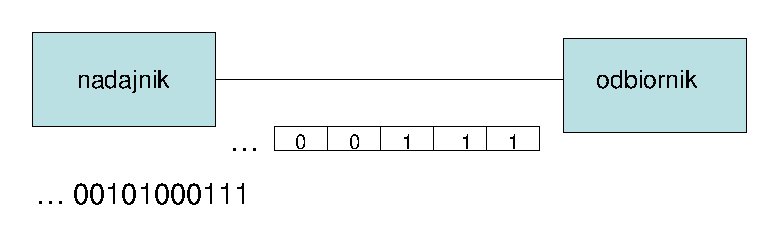
\includegraphics[width=9cm]{./wyklady/RS232_2_1.pdf}
			\item Równoległa - przesyłanie bitów słowa po przyporządkowanej każdemu bitowi linii transmisyjnej (bity przesyłane równolegle, słowa przesyłane szeregowo).\\
			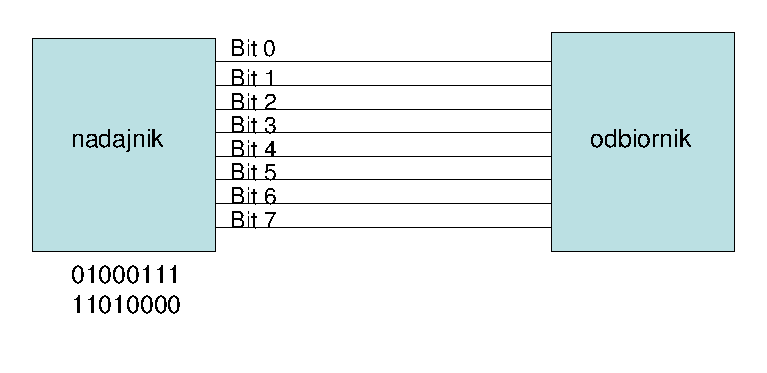
\includegraphics[width=9cm]{./wyklady/RS232_2_2.pdf}
		\end{itemize}
		\subsubsection{Definicje danych}
		\begin{itemize}
			\item "0" - 0V
			\item "1" - 12V
			\item Czas transmisji jednego bitu T - stały, nie większy niż czas propagacji.
			\item $\frac{1}{T}$ - liczba bitów przesyłana w jednostce czasu. Standardowe wartości 110, 150, 300, 600, 1200, 2400 ... [b/s]
			\item Impulsy rozeznające - sprawdzają stan bitów odebranych (następują co T, które narzuca nadawca).
		\end{itemize}
		\subsubsection{Jednostka informacyjna - znak}
		Jednostka informacji o ściśle określonym formacie. Odbiorca dysponuje impulsami próbkującymi, które rozpoznają stan sygnału (odpytują).\\
		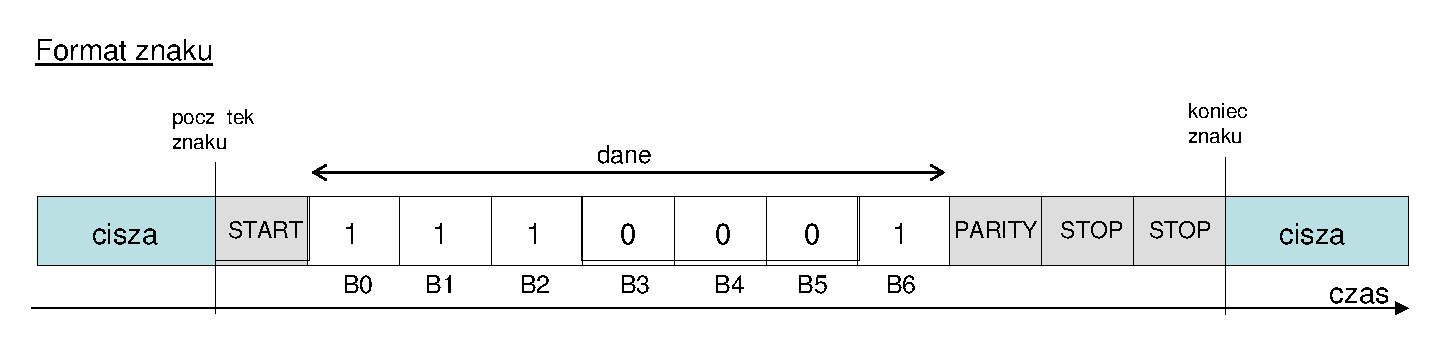
\includegraphics[width=10cm]{./wyklady/RS232_3_2.pdf}\\
		\subsubsection{Przekazywanie konfiguracji}
			Aby nadawca i odbiorca mogli się porozumieć i interpretować znaki w ten sam sposób, muszą zostać tak samo skonfigurowane. Innymi słowy, muszą posiadać ten sam takt nadawania.\\Metody:\\
			\begin{itemize}
				\item dodatkowe łącze
				\item jako element konfiguracji (wykorzystanie generatorów kwarcowych, synchronizm częstotliwościowy)
			\end{itemize}
			Nominalne położenie impulsu = ok. $\frac{1}{2}\times{T}$ - pośrodku, największe bezpieczeństwo próbkowania. Służą do tego układy korekcji fazy impulsu - liczniki, zliczają liczbę impulsów na wejściu i dają 1 na wyjściu.
		\subsubsection{Definicja znaku}
		\begin{itemize}
			\item \textbf{START} - bit kontrolny, znacznik początku (SOF - Start Of Frame) - jałowy z punktu widzenia przesyłanej informacji i służący jedynie w celu synchronizacji. START zapewnia $\frac{n}{2}$ jako stan licznika (fazy impulsu).
			\item \textbf{DANE} - 7-8 bitów (kiedyś też 5-6, obecnie już nieużywane), które są treścią znaku, począwszy od bitu najmniej znaczącego (LSB - least significant bit). Tym bitem jest B0.
			\item \textbf{PARITY} – bit kontroli poprawności znaku, służy jako zabezpieczenie informacji. Może, ale nie musi występować. Jednak decyzja o jego występowaniu ma charakter globalny - dotyczy każdego znaku w danej transmisji. Jego stan określa zasada:
			\begin{itemize}
				\item Kontrola parzystości (Even parity) - polega na sprawdzeniu liczby jedynek na polu danych i ustawieniu bitu kontrolnego na "1" w przypadku nieparzystej liczby jedynek lub na "0" w przypadku parzystej (uzupełnienie do parzystości).
				\item Kontrola nieparzystości (Odd parity) - polega na sprawdzeniu liczby zer na polu danych i ustawieniu bitu kontrolnego na "1" w przypadku nieparzystej liczby zer lub na "0" w przeciwnym przypadku.
				\item Brak kontroli (None)
			\end{itemize}
			Ten bit kontroli pozwala wykryć przekłamanie w transmisji danych pod warunkiem, ze liczba przekłamań jest nieparzysta.
			\item \textbf{STOP} – 1 lub 2 bity kontrolne, znacznik końca znaku.
		\end{itemize}
		\subsubsection{Konwencja nazewnicza rodzajów transmisji}
			[Ilość bitów danych][Rodzaj kontroli][Liczba bitów stopu]\\Przykłady:
			\begin{itemize}
				\item 7E2 - 7 bitów danych, kontrola parzystości, 2 bity stopu (10 bitów + START = 11 bitów)
				\item 8O1 - 8 bitów danych, kontrola nieparzystości, 1 bit stopu (11 bitów)
				\item 8N2 - 8 bitów danych, brak kontroli, 2 bity stopu (11 bitów)
			\end{itemize}
		\subsubsection{Rodzaje transmisji}
		\begin{itemize}
			\item \textbf{Synchroniczna} - elementy informacji wysyłane w takt zegara nadajnika. W ten sposób przesyłane są bity w ramach pojedynczej jednostki informacyjnej.
			\item \textbf{Asynchroniczna} - wysyłanie elementów informacji niesynchronizowane zegarem nadajnika. W ten sposób są wysyłane poszczególne jednostki - ich wprowadzanie nie jest sygnalizowany żadnym sygnałem, więc odstęp między nimi jest dowolny.\\
			Czas trwania bitu nazywa się \emph{odstępem jednostkowym} i oznaczamy go $t_{b}$. Jego odwrotność ($f=\frac{1}{t_{b}}$) określa szybkość transmisji w bodach, gdzie 1 [bd] = 1 [bit/s].
		\end{itemize}
		\subsubsection{Transmisja w RS-232}
		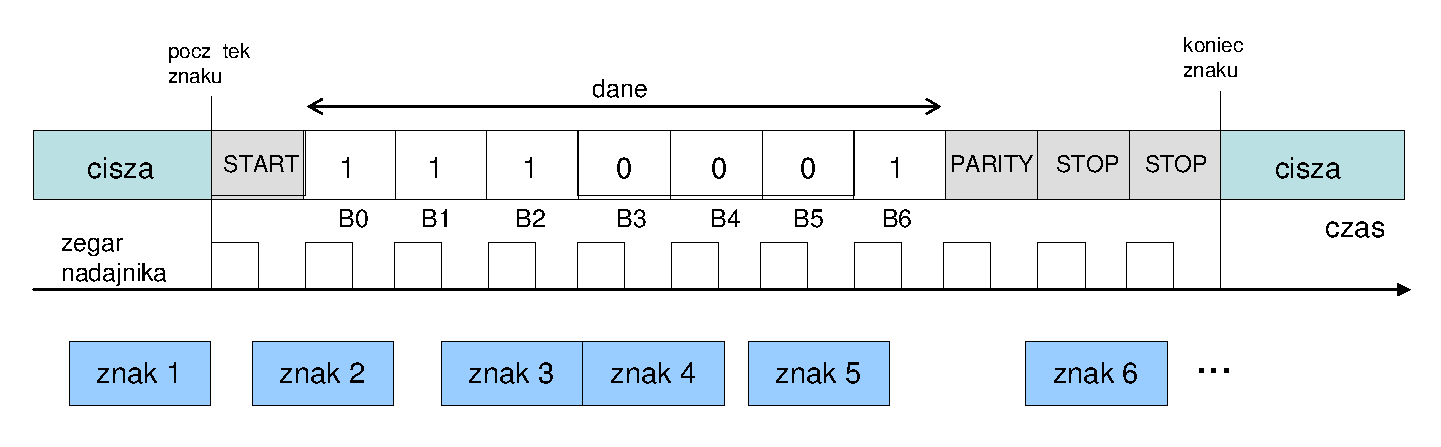
\includegraphics[width=9cm]{./wyklady/RS232_4_1.pdf}
		\begin{itemize}
			\item Synchroniczne wysyłanie bitów
			\item Asynchroniczne wysyłanie znaków
			\begin{itemize}
				\item Polega na wysyłaniu pojedynczych znaków, które mają ścisłe określony format.
				\item Brak sygnału zegarowego określającego momenty wysyłania znaków.
				\item Odstępy między znakami nieokreślone.
			\end{itemize}
		\end{itemize}
		\subsubsection{Tryby transmisji}
		\begin{itemize}
			\item \textbf{Simpleksowa} - jednokierunkowa, z nadajnika do odbiornika.
			\item \textbf{Półdupleksowa} (HDX) - dwukierunkowa, niejednoczesna (w danej chwili czasu jedno urządzenia jest nadajnikiem, a drugie odbiornikiem). Zakłada istnienie tylko jednej linii transmisyjnej. Wymaga konfiguracji (informacja, kto kiedy nadaje).
			\item \textbf{Dupleksowa} (FDX) - dwukierunkowa, jednoczesna (w danej chwili czasu oba urządzenia mogą spełniać rolę nadajnika lub odbiornika). Brak konieczności sprawdzania czy łącze jest wolne oraz mechanizmu rezerwacji łącza.
		\end{itemize}
	\subsection{Komunikacja DTE-DCE - sygnały w porcie RS-232}
	Komunikacja dwóch stacji DTE przez komutowane łącze telefoniczne.\\
	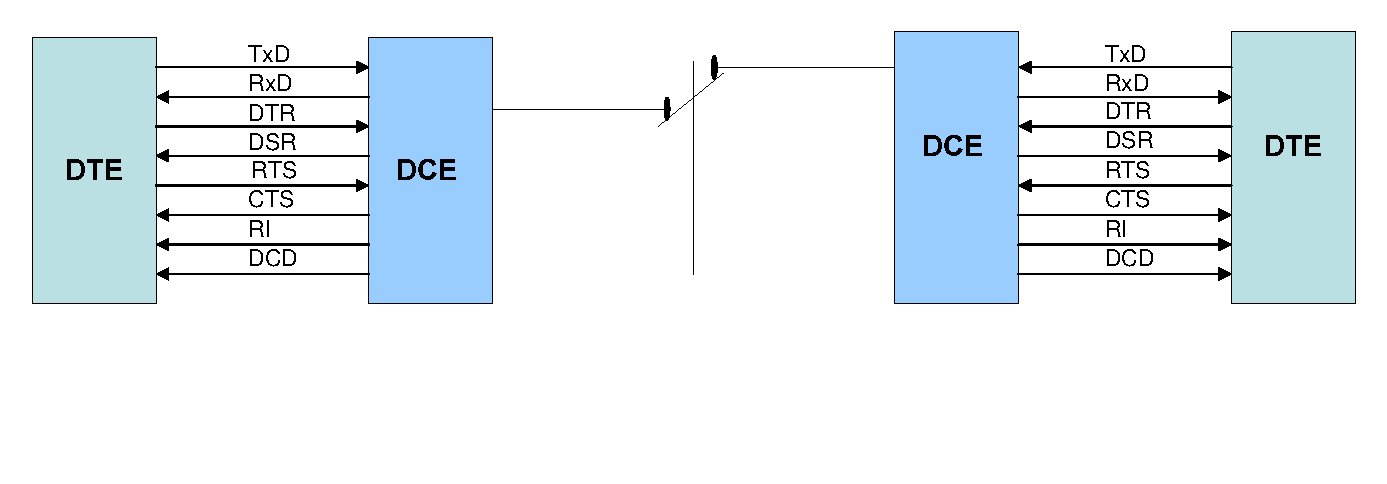
\includegraphics[width=12cm]{./wyklady/RS232_6_1.pdf}\\
	\begin{table}[h]
		\begin{tabular}{|c|c|c|c|c|}
			\hline
			\multicolumn{5}{|c|}{\textbf{Urządzenia}}                        \\ \hline
			\multicolumn{1}{|c|}{DTE} & \multicolumn{2}{|c|}{Data Terminal Equipment}      & \multicolumn{2}{|c|}{Komputer}           \\ \hline
			\multicolumn{1}{|c|}{DCE} & \multicolumn{2}{|c|}{Data Communication Equipment} & \multicolumn{2}{|c|}{Modem}              \\ \hline
			\multicolumn{5}{|c|}{\textbf{Linie} (sygnały)}                   \\ \hline
			\textbf{Skrót} & \textbf{Nazwa}	   & \textbf{Znaczenie} & \textbf{Przeznaczenie} & \textbf{Kierunek} \\ \hline
			TxD & Transmitted Data             & Dane nadawane      & Linia danych		& Wyjście	\\ \hline
			RxD & Received Data                & Dane odbierane     & Linia danych		& Wejście	\\ \hline
			DTR & Data Terminal Ready          & Gotowość DTE       & Linia kontrolna	& Wyjście	\\ \hline
			DSR & Data Set Ready               & Gotowość DCE       & Linia kontrolna	& Wejście	\\ \hline
			RTS & Request to Send              & Żądanie nadawania  & Linia kontrolna	& Wyjście	\\ \hline
			CTS & Clear To Send                & Zgoda na nadawanie & Linia kontrolna	& Wejście	\\ \hline
			RI  & Ring Indicator               & Wskaźnik wywołania & Linia kontrolna   & Wejście	\\ \hline
			DCD & Data Carrier Detected        & Wykrycie nośnej    & Linia kontrolna   & Wejście	\\ \hline
			SG  & Signal Ground                & Masa sygnałowa     & Masa				& ------	\\ \hline
		\end{tabular}
	\end{table}
		\subsubsection{Fazy pracy układu}
		\begin{itemize}
			\item Tryb nawiązywania połączenia
			\item Tryb transmisji danych (wtedy nas interesują dupleksy i inne)
		\end{itemize}
		\subsubsection{Linie w złączu RS-232}
		\begin{itemize}
			\item Linie danych: TxD, RxD
			\item Linie kontrolne: DTR, DSR, RTS, CTS, RI, DCD
		\end{itemize}
	\subsection{Połączenie bezmodemowe DTE-DTE}
	Przykład połączenia dla transmisji dupleksowej.\\
	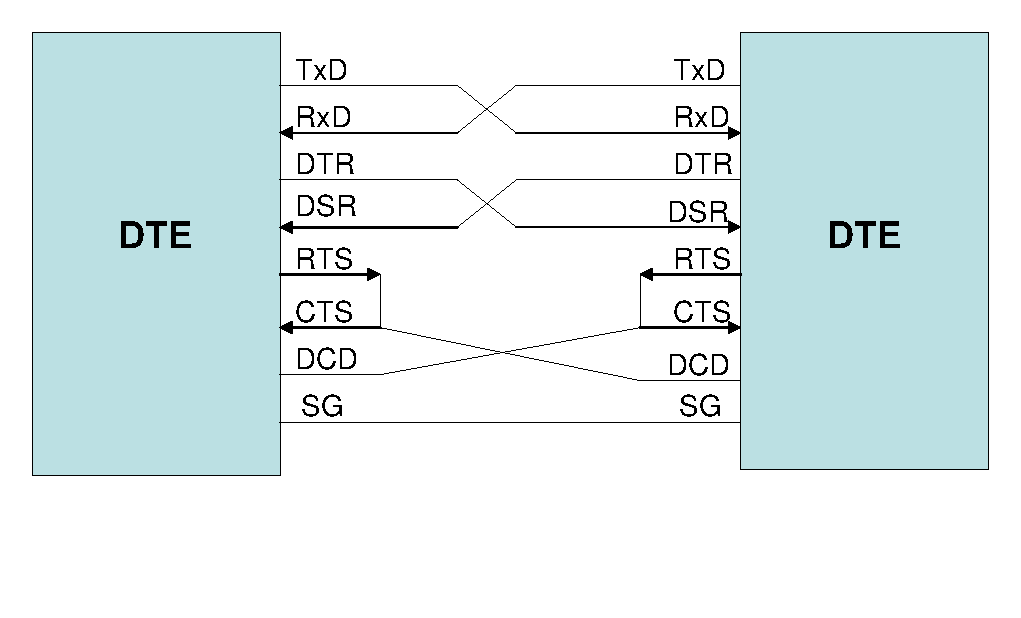
\includegraphics[width=9cm]{./wyklady/RS232_7_1.pdf}
	\begin{itemize}
		\item PG, SG - masa
		\item TxD, RxD - dane
		\item RTS, CTS, DCD, DSR, DTR - sterowanie
	\end{itemize}
	\subsection{Kontrola transmisji: handshake i protokół XON/XOFF}
		\subsubsection{Handshake}
		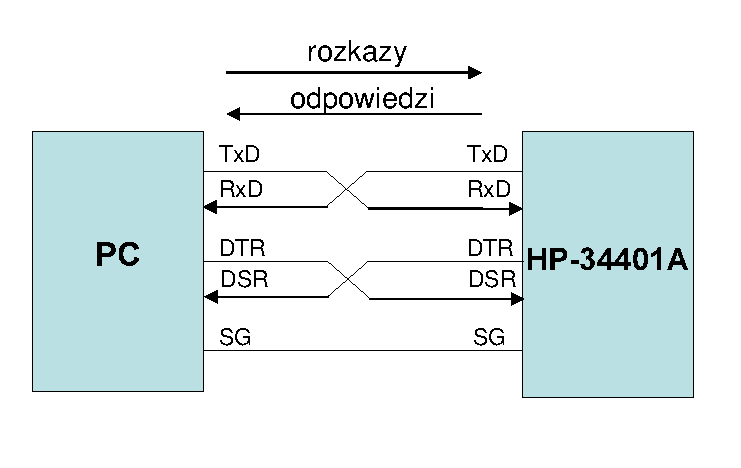
\includegraphics[width=9cm]{./wyklady/RS232_9_1.pdf}
		\begin{itemize}
			\item DTR = 1 - zgoda na nadawanie
			\item DTR = 0 - brak zgody na nadawanie
			\item DTR informuje, czy bufor jest zapełniony. DSR sprawdza go u partnera przed wysłaniem dalszych danych.
			\item Analogiczna sytuacja, kiedy podłączone są RTS i CTS zamiast DTR i DSR. RTS wystawia informację, CTS sprawdza.
		\end{itemize}
		\subsubsection{Protokół XON/XOFF}
		Występuje przy wymianie informacji w trybie dupleksowym. Umożliwia blokowanie i odblokowywanie transmisji danych. Np. drukarka - gdy skończy się papier w trakcie drukowania, przesył jest blokowany, Gdy użytkownik uzupełni papier, transmisja jest wznawiana. Taki protokół XON/OFF nazywany jest programowym (software XON/OFF). {\small Rozwiązanie hardware to transmisja półdupleksowa za pośrednictwem sygnałów w kanale wtórnym.}\\
		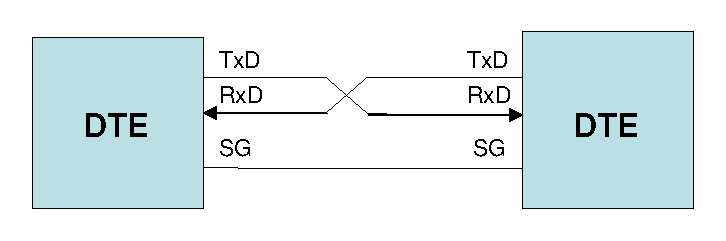
\includegraphics[width=9cm]{./wyklady/RS232_9_2.pdf}
		\begin{itemize}
			\item XON – ASCII 19 (CTRL-S)
			\item XOFF – ASCII 17 (CTRL-Q)
		\end{itemize}
	\subsection{Parametry elektryczne sygnałów}
	Poniżej przestawiono schemat "obwodu stykowego" złożonego ze źródła sygnału, toru transmisyjnego i odbiornika. Parametry zdefiniowano przy założeniu, że szybkość transmisji nie przekracza 20 kbd.
	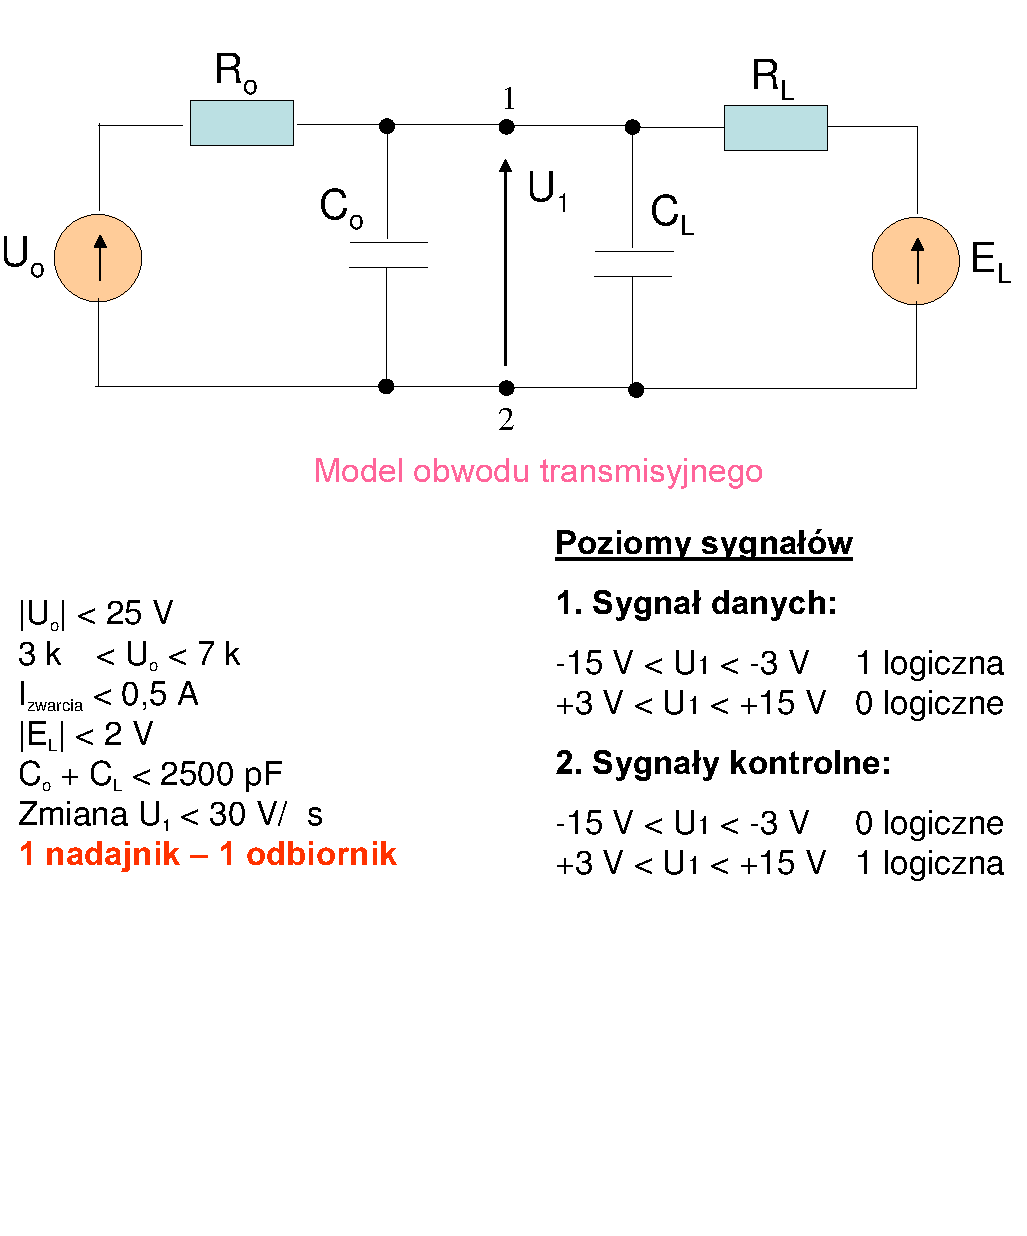
\includegraphics[width=9cm]{./wyklady/RS232_10_1.pdf}\\
	Na rysunku powyżej: kiloomy oraz mikrosekundy.\\
	Wada: jest to obwód represyjny, da się go silnie zakłócić poprzez różnicę potencjałów pomiędzy masami.
	\subsection{Standardy RS-423, RS-422, RS-485}
	Niesymetryczna przesyłanie danych w RS-232C ogranicza szybkość i odległość transmisji, a ponadto nie jest zabezpieczone przed zakłóceniami zewnętrznymi. Aby to polepszyć wymyślono inne standardy.
		\subsubsection{RS-423A}
		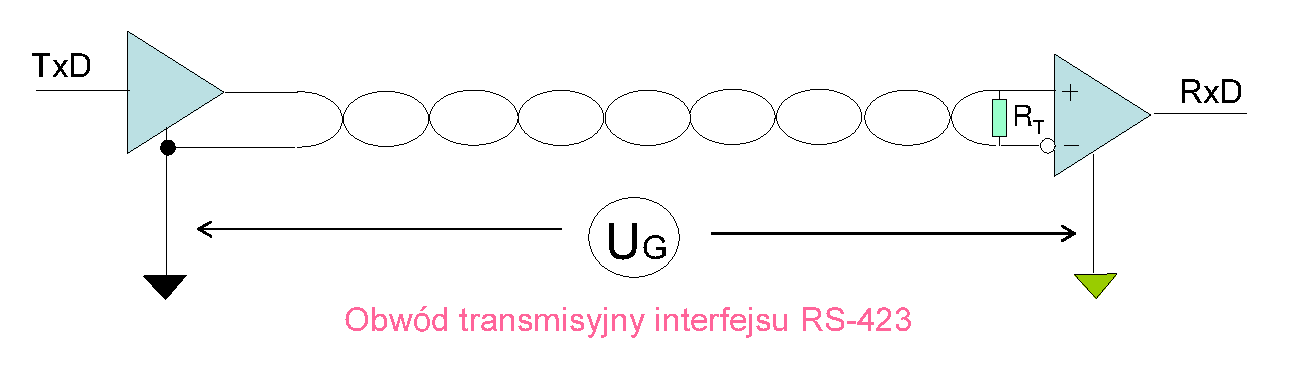
\includegraphics[width=9cm]{./wyklady/RS232_12_1.pdf}
		\begin{itemize}
			\item szybkość do 100 kbd (przy zasięgu do 30 m)
			\item zasięg do 1200 m (przy szybkosci do 3 kbd)
		\end{itemize}
		Standard RS-423A określa elektryczną charakterystykę napięciowego obwodu transmisyjnego złożonego z niesymetrycznego nadajnika oraz symetrycznego (różnicowego) odbiornika. Takie obwody stosuje się do przesyłania sygnałów binarnych pomiędzy DTE i DCE, które reprezentują dane lub funkcje sterujące.\\
		Zastosowanie różnicowego obciążenia pozwala na znaczne zmniejszenie wpływu napięcia wspólnego $U_{G}$ powstałego na wskutek różnicy potencjałów masy nadajnika i odbiornika, jak również przesłuchów między nimi.\\
		Standard wymaga aby dla każdego kierunku transmisji istniał przynajmniej jeden niezależny przewód powrotny.\\
		Typowa prędkość wynosi 100 kb/s przy odległości do 30 m.
		\subsubsection{RS-422A}
		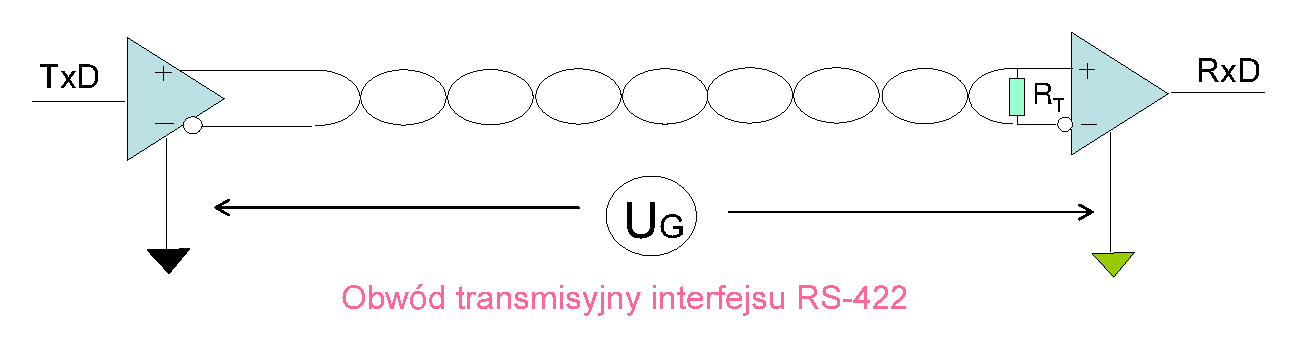
\includegraphics[width=9cm]{./wyklady/RS232_12_2.pdf}
		\begin{itemize}
			\item szybkość do 10 Mbd (przy zasięgu do 100 m)
			\item zasięg do 1200 m (przy szybkości 100 kbd)
		\end{itemize}
		Wykorzystuje pełną symetryzację łącza, zapewnia szybka transmisję w obecności zakłóceń. Standardy RS-423 oraz RS-485 określają symetryczny, zrównoważony system transmisji danych złożony z:
		\begin{itemize}
			\item różnicowego nadajnika
			\item dwuprzewodowego zrównoważonego toru przesyłowego
			\item odbiornika o różnicowym obwodzie wejściowym.
		\end{itemize}
		Standard RS-422A nie wprowadza ograniczeń na minimalną i maksymalną częstotliwość, a jedynie na zależność między szybkością zmian sygnału, a czasem trwania bitu.
		\subsubsection{RS-485A}
		Standard RS-485A jest rozwinięciem RS-422. Łącze RS-485A jest również zrównoważone i symetryczne, przy czym dopuszcza się nie tylko wiele odbiorników, ale i wiele nadajników podłączonych do jednej linii. Nadajniki muszą być trójstanowe.\\
		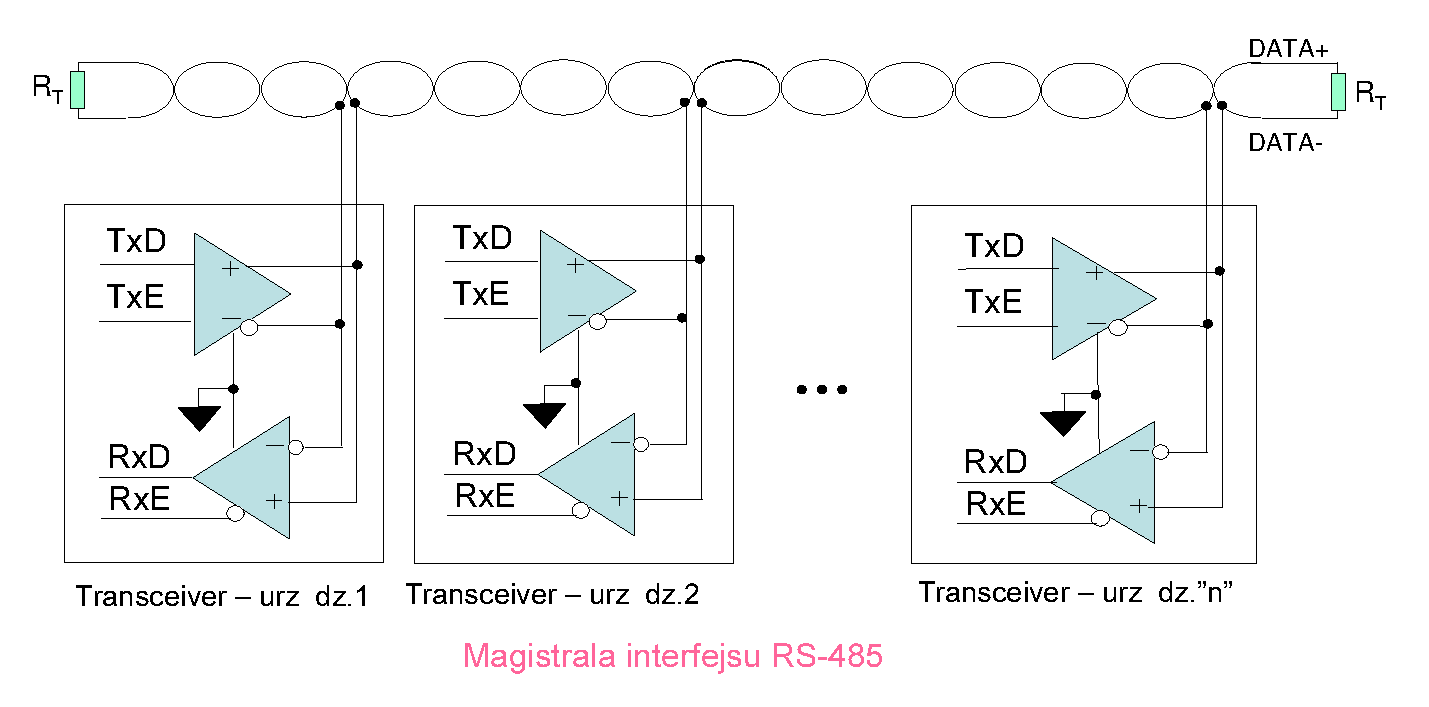
\includegraphics[width=10cm]{./wyklady/RS232_13_1.pdf}
	\subsection{Systemy komunikacyjne oparte na łączu znakowym}
		\subsubsection{System oparty na szeregowym łączu znakowym}
		Podłączenie urządzenia RS-232 do portu COM z pom. int. RS-485\\
		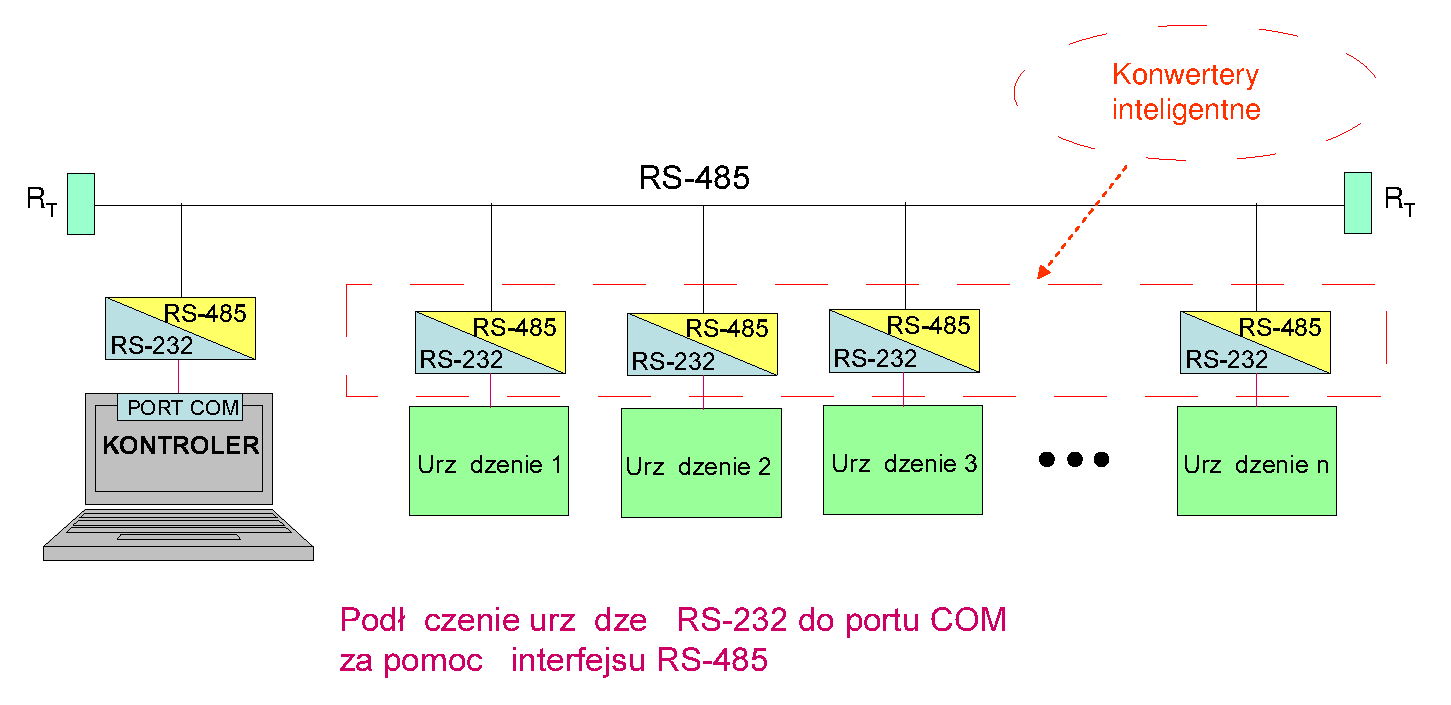
\includegraphics[width=9cm]{./wyklady/RS232_14_1.pdf}\\
		R\tiny T\normalsize - Rezystory zabezpieczające przed niekorzystnym odbiciem fali (tzw. Terminatory).\\
		\textbf{Problem}: dostęp do magistrali kontrolera i urządzeń systemu\\
		\textbf{Rozwiązanie}: Implementacja protokołu komunikacyjnego (warstwa łącza danych). Komputer zarządza innymi urządzeniami w całym systemie. Do zbudowania tego wystarczają proste przejściówki do zmian sygnałów.\\
		\textbf{Komunikacja}:
		\begin{itemize}
			\item Selekcja urządzenia kontrolującego (master) - generuje on rozgłoszenie (broadcast) do wszystkich urządzeń i zbiera dane.
			\item Selekcja urządzenia odbierającego - konieczna gdy wiele urządzeń chce przesłać odpowiedź do mastera, co może powodować konflikt.
			\begin{itemize}
				\item nadanie identyfikatorów (adresacja urządzeń)
				\item zastosowanie przejściówek - są inteligentne i odpowiadają za dostęp do urządzenia.
			\end{itemize}
		\end{itemize}
		\subsubsection{System oparty na łączu znakowym}
		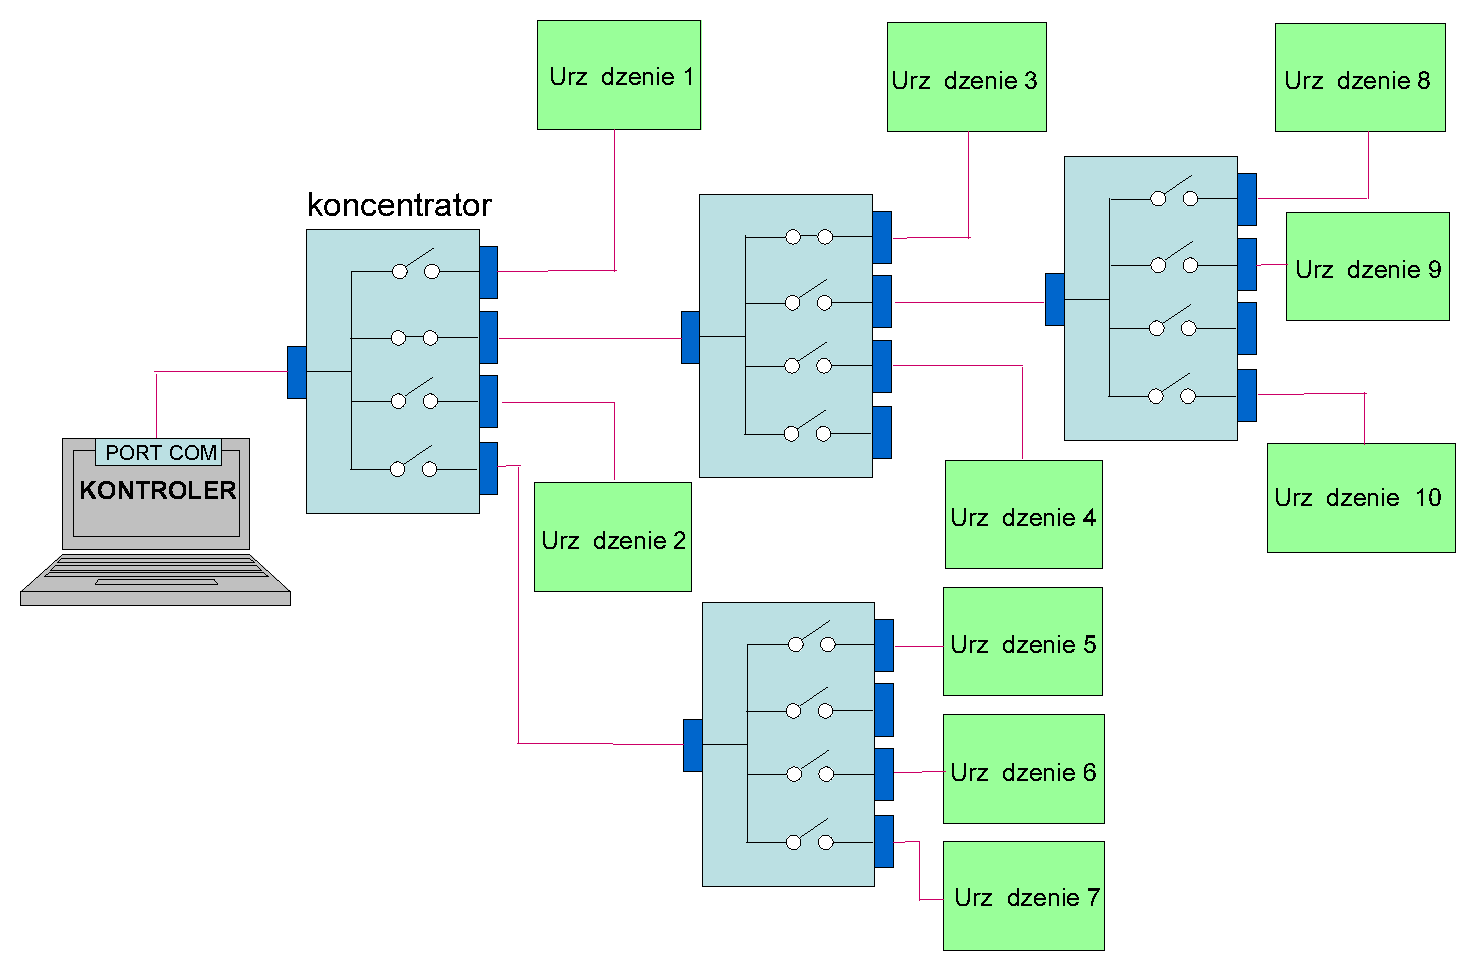
\includegraphics[width=10cm]{./wyklady/RS232_15_1.pdf}\\
		Koncentrator zawiera 4 klucze portu RS. Dostęp jest tylko do jednego wyjścia naraz.\\
		\textbf{Kaskadowe połączenie} - przełącznik podłączony do przełącznika. Pojawia się problem wyboru drogi do urządzenia, która musi być znana. Koncentratory muszą mieć informacje o \textbf{mapie urządzeń}.
	\subsection{System MODBUS}
		Interfejs MODBUS został opracowany w firmie Modicon i jest przyjętym standardem w dla asynchronicznej, znakowej wymiany informacji pomiędzy urządzeniami systemów pomiarowo-kontrolnych.
		\subsubsection{Charakterystyka}
			\begin{itemize}
				\item Reguła dostępu do łącza na zasadzie Master-Slave. 
				\item Zabezpieczenie przesyłanych komunikatów przed błędami
				\item Potwierdzenie wykonania rozkazów zdalnych i sygnalizacja błędów
				\item Mechanizmy zabezpieczające przed zawieszeniem systemu
				\item Wykorzystanie asynchronicznej transmisji znakowej zgodnej z RS-232C
			\end{itemize}
		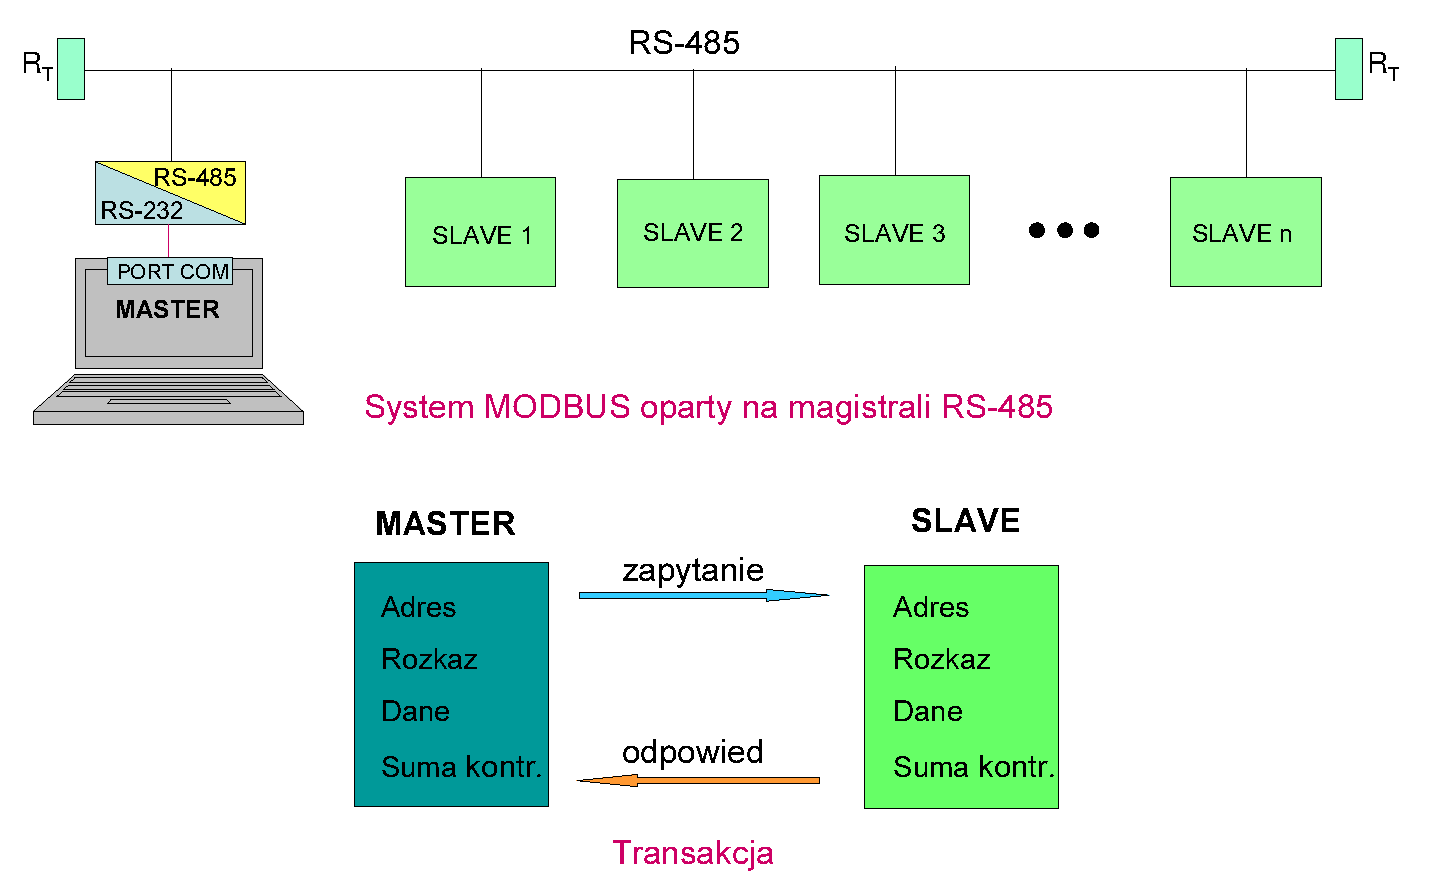
\includegraphics[width=9cm]{./wyklady/RS232_16_1.pdf}\\
		\subsubsection{Transakcja}
		Jedno urządzenie może inicjować transakcje (master), a pozostałe (slave) odpowiadają jedynie na zapytania mastera. Transakcja składa się z polecenia (query) wysyłanego z master do slave oraz z odpowiedzi (response) przesyłanej ze slave do master. Odpowiedź zawiera dane żądane przez master lub potwierdzenie realizacji jego połączenia. Wykrycie końca kończy fazę w której następuje przekazanie łącza masterowi.\\
		\subsubsection{Format wiadomości}
		Dotyczy zarówno poleceń jednostki nadrzędnej, jak i odpowiedzi podrzędnych.
		\begin{itemize}
			\item Adres
			\item Kod funkcji reprezentujący rozkaz, pierwszy bit rozkazu oznacza jego rodzaj. 0 - normalny, 1 - szczególny.
			\item Dane
			\item Kontrola błędów (dla pracy w warunkach przemysłowych)
		\end{itemize}
		W przypadku odpowiedzi odpowiednio w polach znajdują się:
		\begin{itemize}
			\item Adres (swój, slave'a, do kontroli poprawności)
			\item Pole potwierdzenia realizacji rozkazu
			\item Dane żądane przez master
			\item Kontrola błędów
		\end{itemize}
		\subsubsection{Rodzaje transakcji}
			\begin{itemize}
				\item \textbf{Adresowana} - przeznaczona dla pojedynczej jednostki slave
				\item \textbf{Rozgłoszeniowa} (broadcast) - wysyłana do wszystkich jednostek podrzędnych. Na ten rodzaj polecenia jednostki nie przesyłają odpowiedzi.
			\end{itemize}
		\subsubsection{Rodzaje odpowiedzi}
			\begin{itemize}
				\item \textbf{Normalna} - w przypadku poprawnego wykonania polecenia.
				\item \textbf{Szczególna} - jeżeli slave wykryje błąd przy odbiorze wiadomości lub nie jest w stanie wykonać polecenia, to przygotowuje specjalny komunikat o wystąpieniu błędu i przesyła jako odpowiedź. W przypadku tej wiadomości jest ona \textbf{powiększona} o 128 - miejsce na kod błędu.
			\end{itemize}
		\subsubsection{Parametry protokołu}
			\begin{itemize}
				\item Reguła dostępu do łącza: Master-Slave
				\item Zakres adresów: 1 - 247 (identyfikatory slave'ów)
				\item Adres rozgłoszeniowy: 0, rozpoznawany przez wszystkie slave'y
				\item Kontrola błędów: LRC/CRC, ograniczenie czasowe odpowiedzi
				\item Wymagana ciągłość przesyłania znaków w ramce
			\end{itemize}
		\subsubsection{Ramka w systemie MODBUS}
			W systemie MODBUS wiadomości są zorganizowane w ramki o określonym początku i końcu. Umożliwia do odbiornikowi odrzucenie ramek niekompletnych i sygnalizację błędów.
		\subsubsection{Rodzaje transmisji ramek}
			\begin{itemize}
				\item ASCII
				\item RTU
			\end{itemize}
		\subsubsection{Ramka w trybie ASCII}
			Każdy bajt wiadomości przesyłany jest w postaci dwóch znaków ASCII. Zaletą tego rozwiązania jest to, że pozwala na długie odstępy między znakami (1 s) bez powodowania błędów.\\\\\textbf{Format znaku}\\
			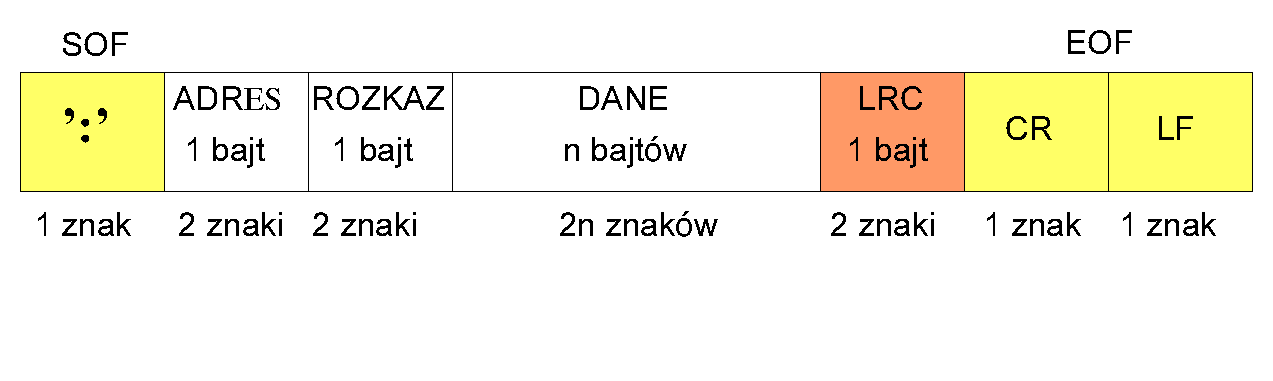
\includegraphics[width=10cm]{./wyklady/RS232_18_1.pdf}
			\begin{itemize}
				\item System kodowania: heksadecymalny, znaki ASCII 0-9, A-F. Jeden znak heksadecymalny zawarty jest w każdym znaku ASCII wiadomości.
				\item Jednostka informacyjna: ograniczona znakami start (na początku) i stop (na końcu), 10-bitowa.
				\item Znacznikiem początku ramki jest znak dwukropka (":" - ASCII 3Ah).
				\item Dopuszczalne znaki dla pozostałych pól (poza znacznikiem końca ramki) to 0-9, A-F.
				\item Pole funkcji: dwa znaki w trybie ASCII
				\item Podsumowując: wykorzystujemy 2 znaki heksadecymalne do przesyłu 1go znaku ASCII. Dzielimy ten na dwie części i przesyłamy w dwóch pakietach po 10 bitów.
				\item Urządzenie po wykryciu znacznika początku sprawdza czy pole adresowe zawiera jego własny adres. Jeżeli tak, to odczytuje zawartość pola funkcji i pola danych.
				\item Pole kontrolne LRC (1-bitowe) zabezpiecza część informacyjną. Sumuje cześć informacyjną bajtu i uzupełnia do 2.
				\item Ramka kończy się przesłaniem dwóch znaków: CR i LF.
				\item Ramkę kończy przerwa czasowa trwająca co najmniej $3.5\times$(długości znaku)
				\item Ramki muszą być przesyłane w postaci ciągłej, tzn. odstęp między kolejnymi znakami tworzącymi ramkę nie może być większy niż $1.5\times$(długości znaku).
			\end{itemize}
			Stosowane jest zabezpieczenie części informacyjnej ramki kodem LRC (Longitudinal Redundancy Check).
		\subsubsection{Ramka w trybie RTU}
			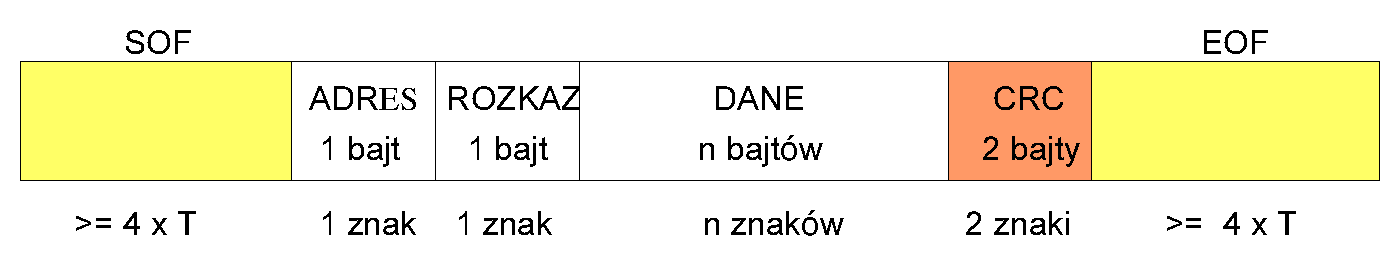
\includegraphics[width=10cm]{./wyklady/RS232_18_2.pdf}\\
			W trybie RTU wiadomości zaczynają się odstępem czasowym trwającym minimum $3.5\times$(\emph{czas trwania pojedynczego znaku}), w którym panuje cisza na łączu (można to zrealizować np. przez odmierzanie czasu trwania znaku przy zadanej na łączu szybkości bodowej).
			\begin{itemize}
				\item Pierwszym polem informacyjnym jest adres urządzenia
				\item Dopuszczalne znaki w ramach pól ramki: 0-9, A-F
				\item Zakres kodów operacji: 1 - 255
				\item Urządzenia stale monitorują magistralę. Jak adres odebrany w wiadomości zgadza się z ich własnym, to lecą dalej.
				\item Ramkę kończy przerwa czasowa trwająca co najmniej $3.5\times$(długości znaku)
				\item W przypadku gdy nowa wiadomość pojawia się przed upływem niezbędnej przerwy to będzie ona potraktowana jako kontynuacja poprzedniej wiadomości. Doprowadzi to do błędu sumy kontrolnej.
				\item Ramki muszą być przesyłane w postaci ciągłej, tzn. odstęp między kolejnymi znakami tworzącymi ramkę nie może być większy niż $1.5\times$(długości znaku).
				\item Przekroczenie odstępu powoduje uznanie ramki za niekompletną i błędną.
				\item Kontrola danych typu CRC - 2-bajtowe, silniejsze niż LRC.
			\end{itemize}
		\subsubsection{Warstwa fizyczna}
		\begin{itemize}
			\item Asynchroniczna transmisja znakowa
			\item Formaty znaków
			\begin{itemize}
				\item Tryb ASCII: 7E1, 7O1, 7N2
				\item Tryb RTU: 8E1, 8O1, 8N2
			\end{itemize}
			\item Szybkość: od 1200 bd do 19200 bd
			\item Rodzaj łącza:
			\begin{itemize}
				\item Magistrala RS-485
				\item Multipleksowany RS-232
			\end{itemize}
			\item Rodzaj transmisji (zależny od łącza):
			\begin{itemize}
				\item różnicowa dla RS-485
				\item odniesiona do masy dla RS-232
			\end{itemize}
		\end{itemize}
	\subsection{Kontroler RS-232 w komputerze PC}
	
\section{USB – Uniwersalny interfejs szeregowy}
	\subsection{Co to jest?}
	\subsection{Parametry}
	Dla USB 1.1 oraz 2.0
	\begin{itemize}
		\item Szybkość transmisji: 12 Mb/s (1.1), 480 Mb/s (2.0)
		\item Złożoność kontrolera w stacji host: 10000 bramek
		\item Złożoność kontrolera w urządzeniu: 1500 do 2000 bramek
	\end{itemize}
	\subsection{Charakterystyka systemu USB}
		\subsubsection{Podstawowe właściwości interfejsu USB}
		\begin{itemize}
			\item \textbf{Gorące podłączenie} - włączanie/wyłączanie urządzeń bez wyłączania systemu.
			\item \textbf{Jeden typ złącza} - złącze typu A w koncentratorze i B w urządzeniu.
			\item \textbf{Duża liczba podłączanych urządzeń} - maksymalnie do 127
			\item \textbf{Różne szybkości transmisji} - mała: 1,5 Mb/s, pełna: 12 Mb/s, wysoka: 480 Mb/s
			\item \textbf{Zasilanie} - system dystrybucji zasilania: 5V/500 mA, zawieszenie, wznowienie, wake-up
			\item \textbf{Protokół komunikacyjny, detekcja błędów} - pakietowy z kontrolą poprawności przesyłu
			\item \textbf{Transfery USB} - 4 typy transferów:
				\begin{itemize}
					\item kontrolny
					\item masowy
					\item przerwaniowy
					\item izochroniczny
				\end{itemize}
			\item \textbf{Niski koszt} - nieduża złożoność układów interfejsowych
			\item \textbf{Schemat blokowy systemu USB}\\
			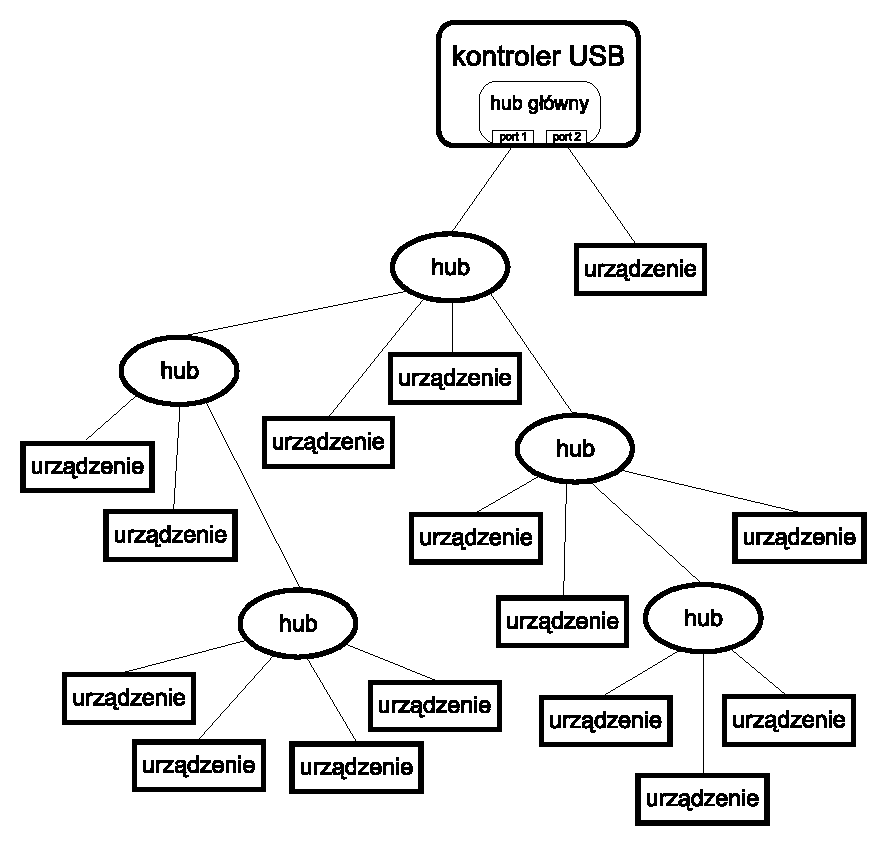
\includegraphics[width=10cm]{./wyklady/USB_6_1.pdf}
		\end{itemize}
		\subsubsection{Środowisko sygnałowe i fizyczne}
			\textbf{Obwód transmisyjny w standardzie USB}\\
			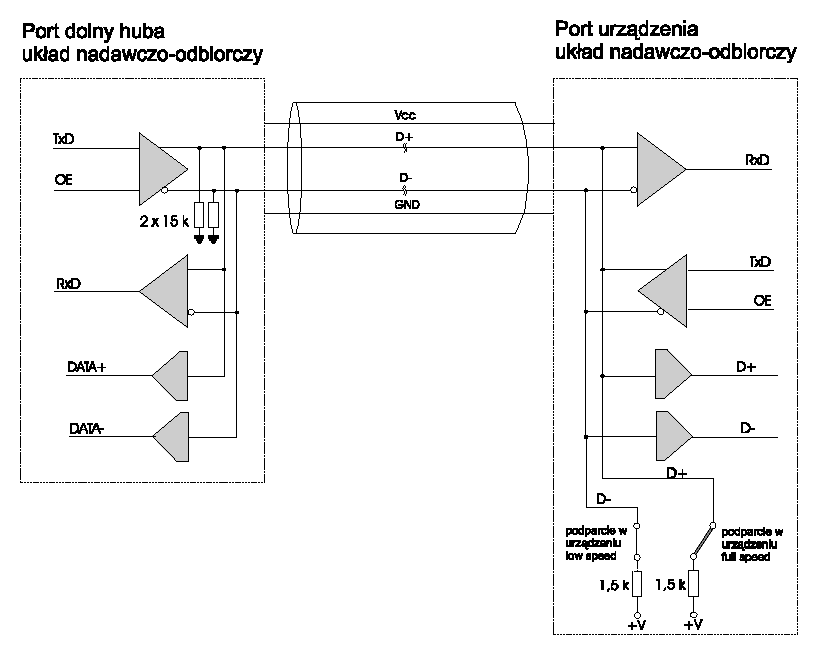
\includegraphics[width=10cm]{./wyklady/USB_7_1.pdf}
			\textbf{Stany magistrali USB}\\
			\begin{itemize}
				\item Logiczne „1” w obwodzie różnicowym (D+) - (D-) $>$ 200 mV
				\item Logiczne „0” w obwodzie różnicowym (D+) - (D-) $<$ -200 mV
				\item Plus 9 innych stanów
			\end{itemize}
			\textbf{Kodowanie NRZI ze wstawianiem bitu synchronizującego}\\
			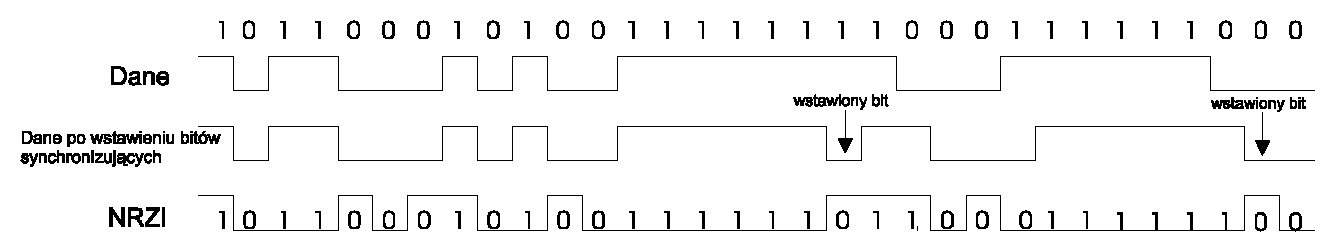
\includegraphics[width=15cm]{./wyklady/USB_9_1.pdf}\\\\
			\textbf{Podstawowy kabel do podłączenia urządzenia USB}\\
			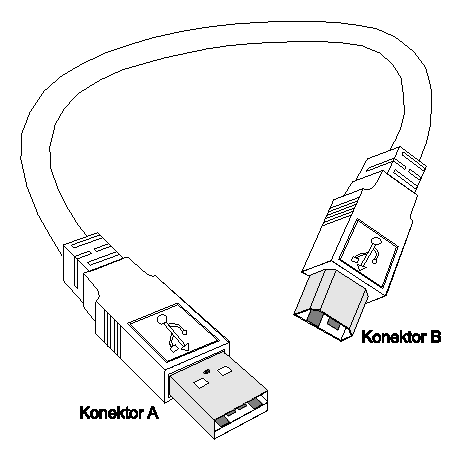
\includegraphics[width=6cm]{./wyklady/USB_10_1.pdf}
			\begin{itemize}
				\item Konektor A – strona portu dolnego (hub)
				\item Konektor B – strona portu górnego (urządzenie)
			\end{itemize}
			\begin{table}[h]
				\begin{tabular}{|c|c|c|}
					\hline
					\textbf{Nr kontaktu}	& \textbf{Nazwa sygnału}	& \textbf{Kolor przewodu w kablu} \\ \hline
					1 						& Vcc						& Czerwony		\\ \hline
					2 						& +DATA						& Biały			\\ \hline
					3 						& -DATA						& Zielony		\\ \hline
					4 						& GND						& Czarny		\\ \hline
				\end{tabular}
			\end{table}
			\textbf{Właściwości}
			\begin{itemize}
				\item Kabel „low speed”
				\begin{itemize}
					\item nieekranowany
					\item dwie, nie skręcane pary przewodów: dla danych (28 AWG) i zasilania (20-28 AWG)
				\end{itemize}
				\item Kabel „full speed i high speed”
				\begin{itemize}
					\item ekranowana para skręcana (28 AWG) dla danych
					\item nieekranowana para (20-28 AWG) dla zasilania
				\end{itemize}
				\item Czas propagacji sygnału w kablu: $<$ 30 ns
			\end{itemize}
		\subsubsection{Ramki i mikro ramki}
			\textbf{Ramki i mikroramki w standardzie USB}\\
			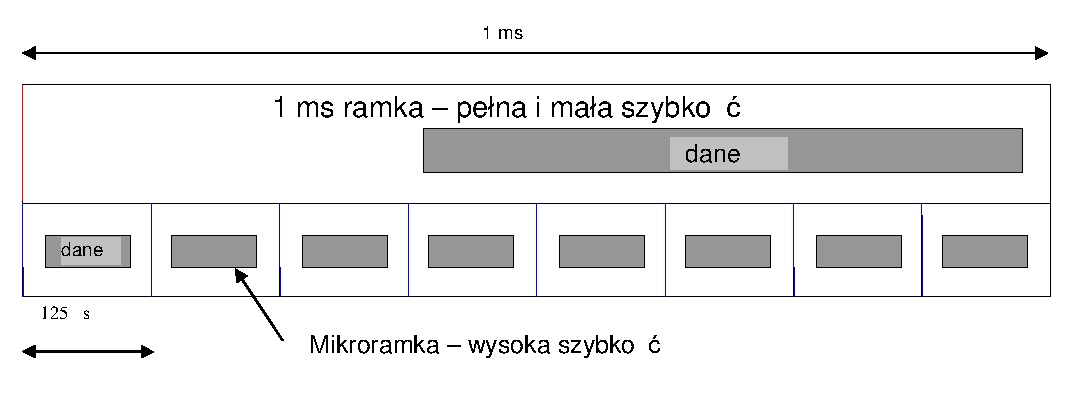
\includegraphics[width=10cm]{./wyklady/USB_11_1.pdf}\\
			\textbf{Właściwości}
			\begin{itemize}
				\item Pełna szybkość transmisji
				\begin{itemize}
					\item Max rozmiar ramki w bitach: 1 ms x 1/12 Mhz = 12000 bitów
					\item Max rozmiar ramki w bajtach: 12000 : 8 = 1500
				\end{itemize}
				\item Mała szybkość transmisji
				\begin{itemize}
					\item Max rozmiar ramki w bitach: 1 ms x 1/1,5 Mhz = 1500 bitów
					\item Max rozmiar ramki w bajtach: 1500 : 8 = 187
				\end{itemize}
				\item Mikroramka 125 $\mu s$
				\begin{itemize}
					\item Mikroramka trwa 125 $\mu s$
					\item Na 1 ramkę przypada 8 mikroramek
				\end{itemize}
				\item Wysoka prędkość transmisji - Szybkość transmisji w mikroramce wynosi 480 Mhz.
			\end{itemize}
		\subsubsection{Model komunikacyjny}
		\textbf{Warstwowy model komunikacyjny}\\
		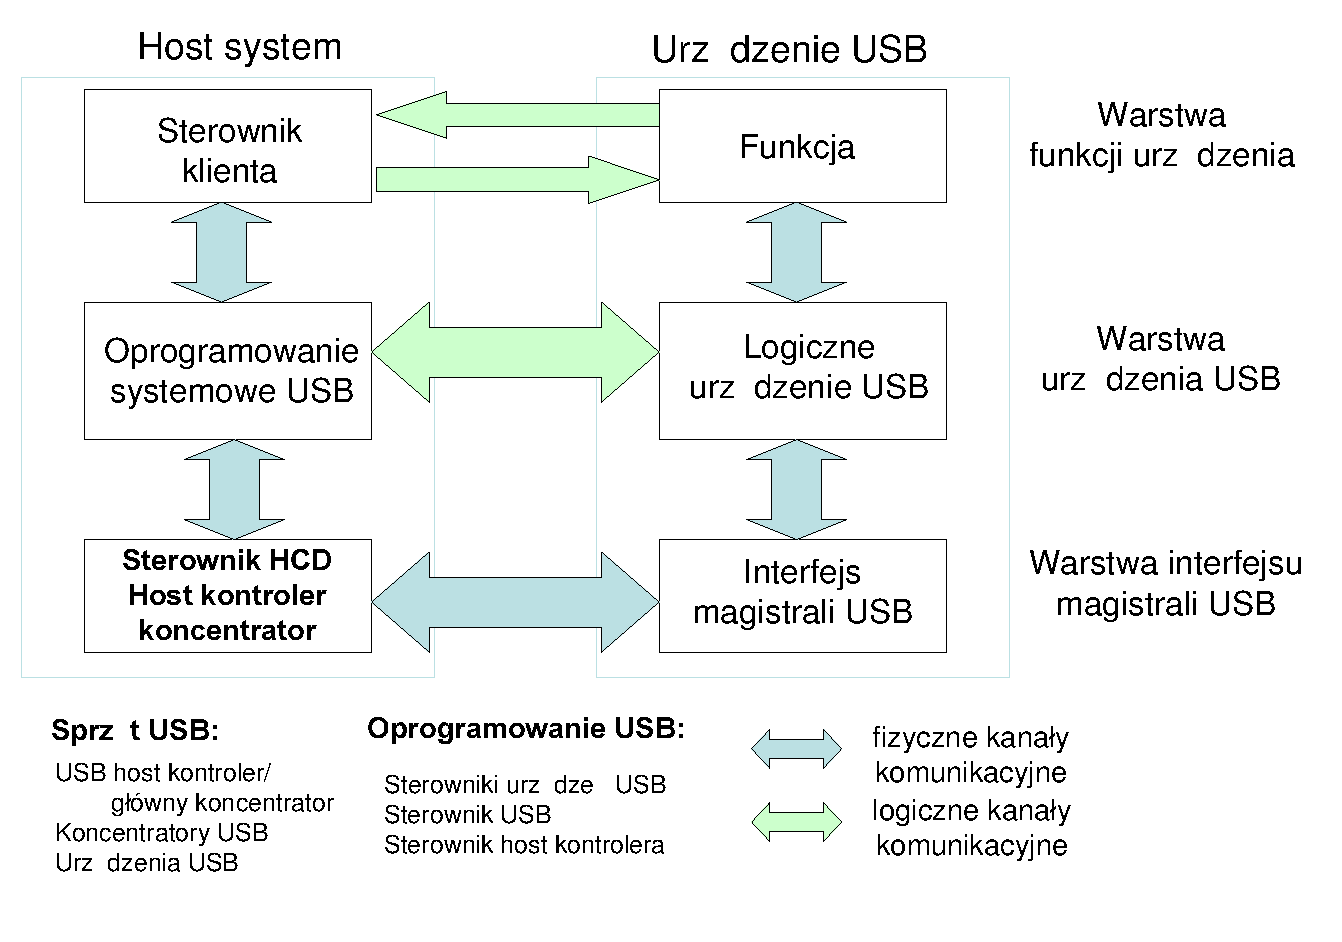
\includegraphics[width=10cm]{./wyklady/USB_12_1.pdf}\\\\
		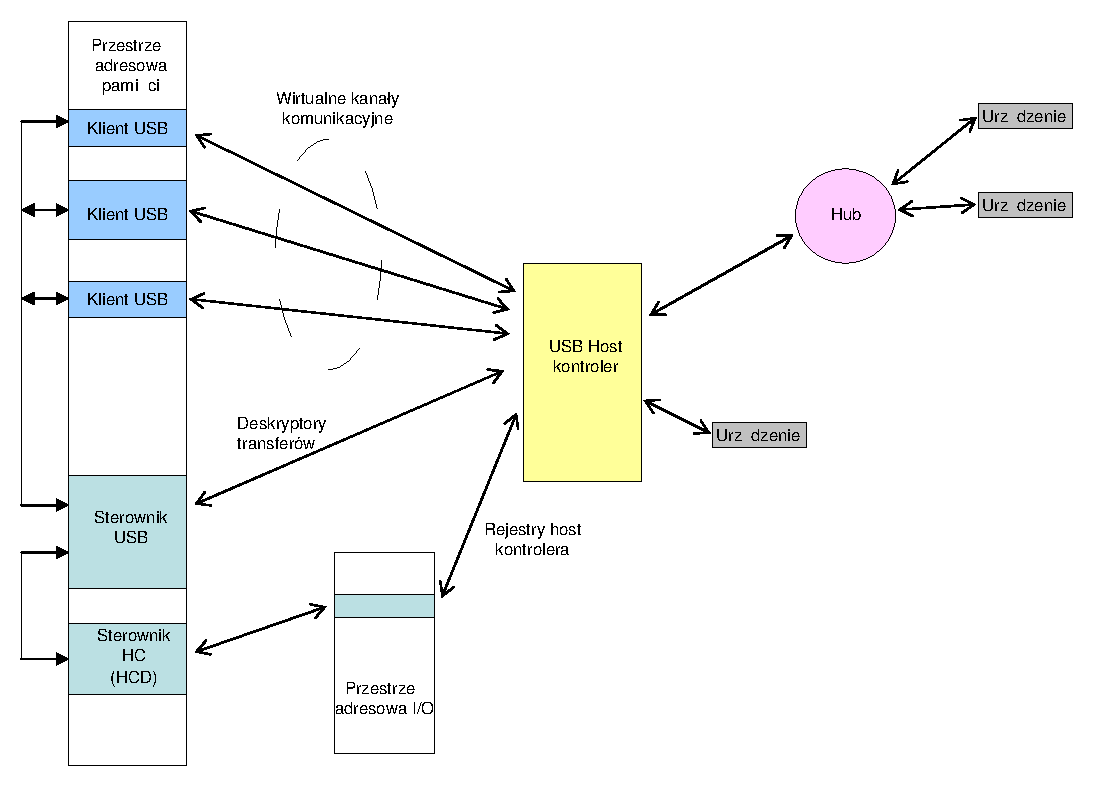
\includegraphics[width=10cm]{./wyklady/USB_13_1.pdf}\\
		\subsubsection{Transfery USB}
		\begin{itemize}
			\item Kontrolny (control transfer) - time delivery accuracy + quality delivery accuracy
			\item Masowy (interrupt transfer) - time delivery accuracy + quality delivery accuracy
			\item Przerwaniowy (bulk transfer) - quality delivery accuracy
			\item Izochroniczny (isochronous transfer) - time delivery accuracy
		\end{itemize}
		\begin{itemize}
			\item Transfery kontrolny i masowy – aperiodyczne
			\item Transfery przerwaniowy i izochroniczny - periodyczne
		\end{itemize}
		\subsubsection{Stany urządzenia USB}
		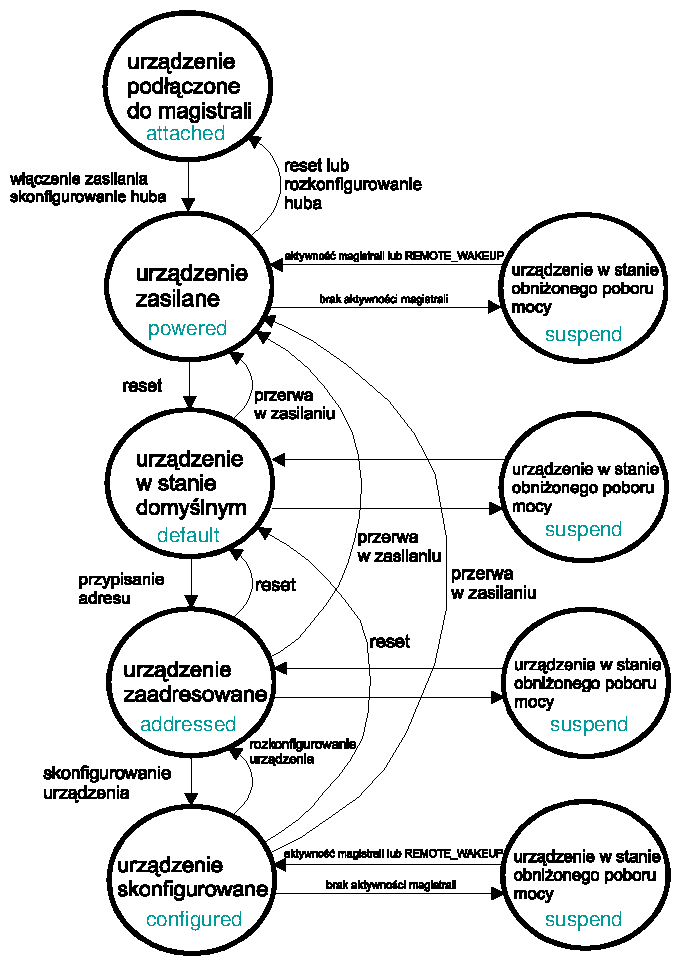
\includegraphics[width=10cm]{./wyklady/USB_16_1.pdf}
		\subsubsection{Hub w systemie USB}
		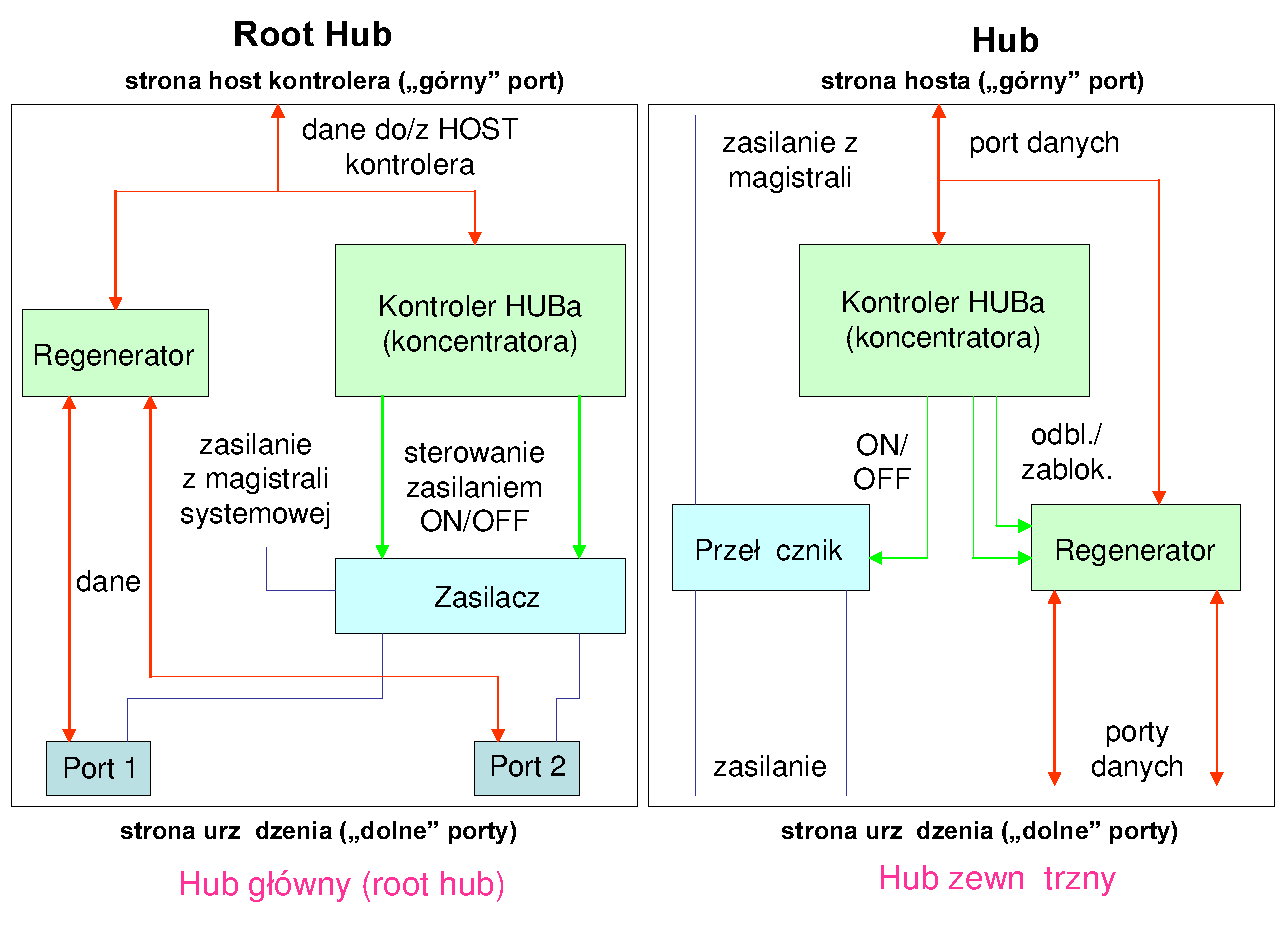
\includegraphics[width=10cm]{./wyklady/USB_17_1.pdf}
	
\subsection{Protokół komunikacyjny}
	\subsubsection{Właściwości}
	\begin{itemize}
		\item Komunikacja z urządzeniami USB za pomocą ramek o długości maksymalnej 1 ms.\\
		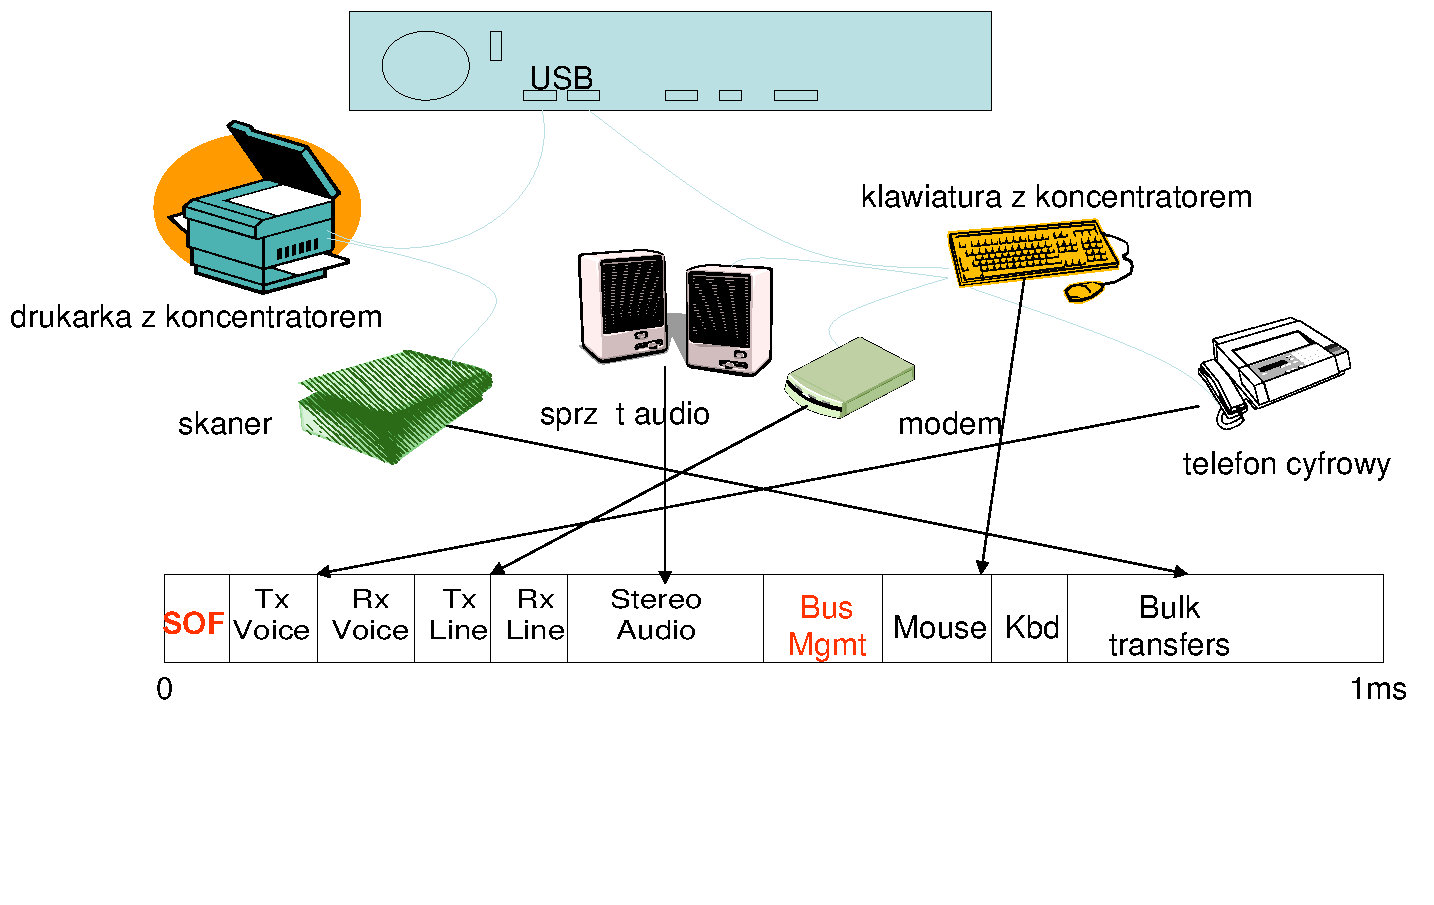
\includegraphics[width=10cm]{./wyklady/USB_18_1.pdf}
		\item Pakietowa struktura komunikatów\\
		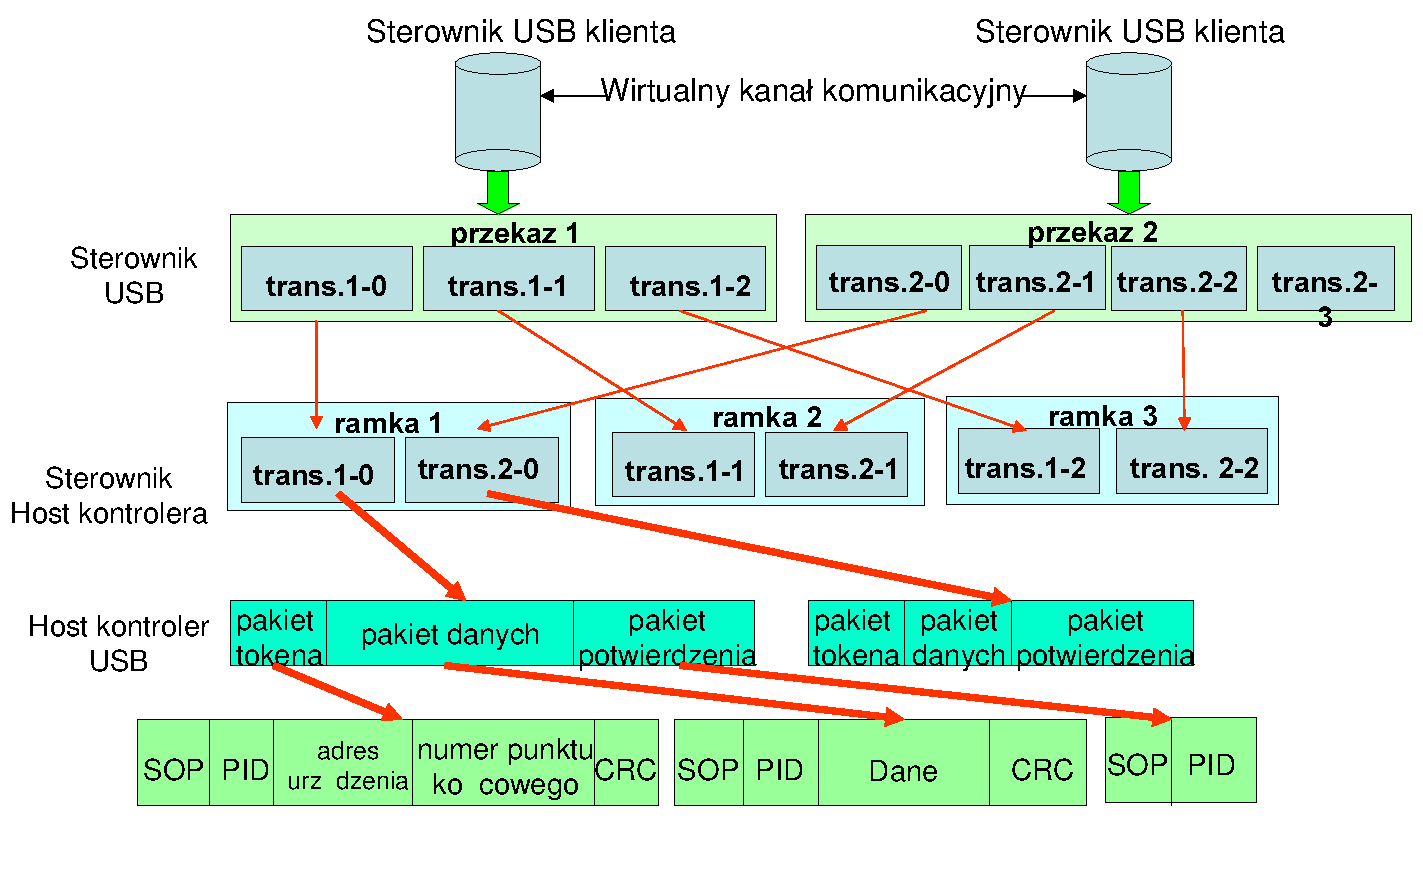
\includegraphics[width=10cm]{./wyklady/USB_19_1.pdf}\\
		Struktura bloków komunikacyjnych w USB
	\end{itemize}
	\subsubsection{Format i typy pakietów USB}
	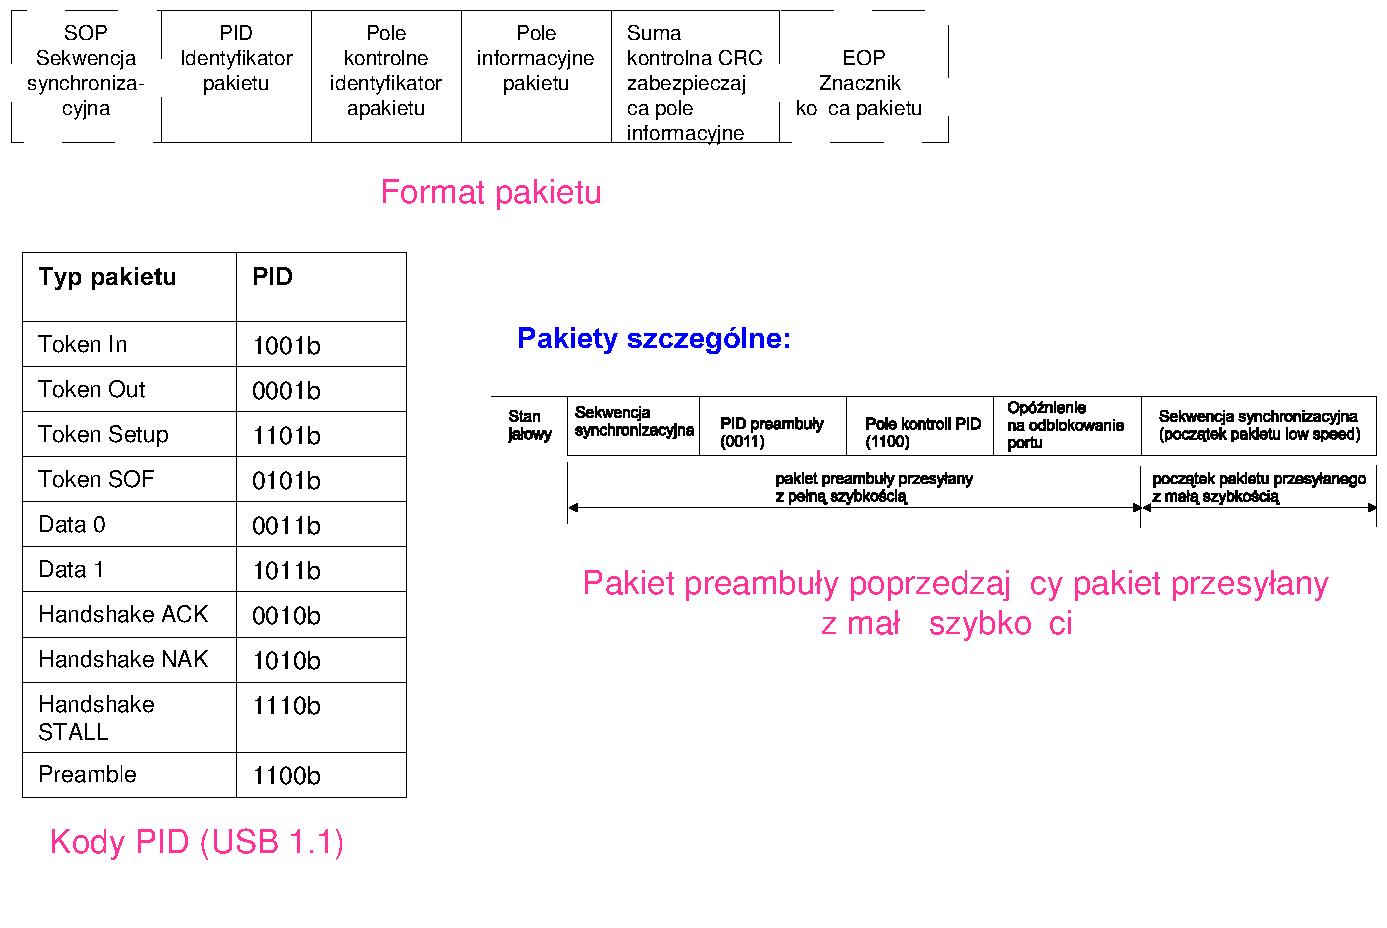
\includegraphics[width=10cm]{./wyklady/USB_20_1.pdf}
	\subsubsection{Reakcja na błędy}
	Wykrywanie błędów i kontrola transmisji\\
	\begin{itemize}
		\item Kontrola poprawności pakietów (zabezpieczenie pola PID, CRC)
		\item Reakcja na fałszywy znacznik końca pakietu (\emph{false EOP})
		\item Ograniczenie czasowe oczekiwania na odpowiedź
		\item Przełączanie kolejnych pakietów danych (mechanizm \emph{data toogle})
		\item Wykrywanie transakcji występujących po zakończeniu ramki (tzw. „paplanie” – \emph{babble})
		\item Wykrywanie braku aktywności magistrali (LOA – \emph{Loss Of Activity})
	\end{itemize}
	\subsubsection{Czas obiegu (\emph{round trip delay})}
	Ograniczenie czasowe oczekiwania na odpowiedź. Poniżej połączenie urządzenia z hostem przez 5 hubów – najgorszy przypadek.\\
	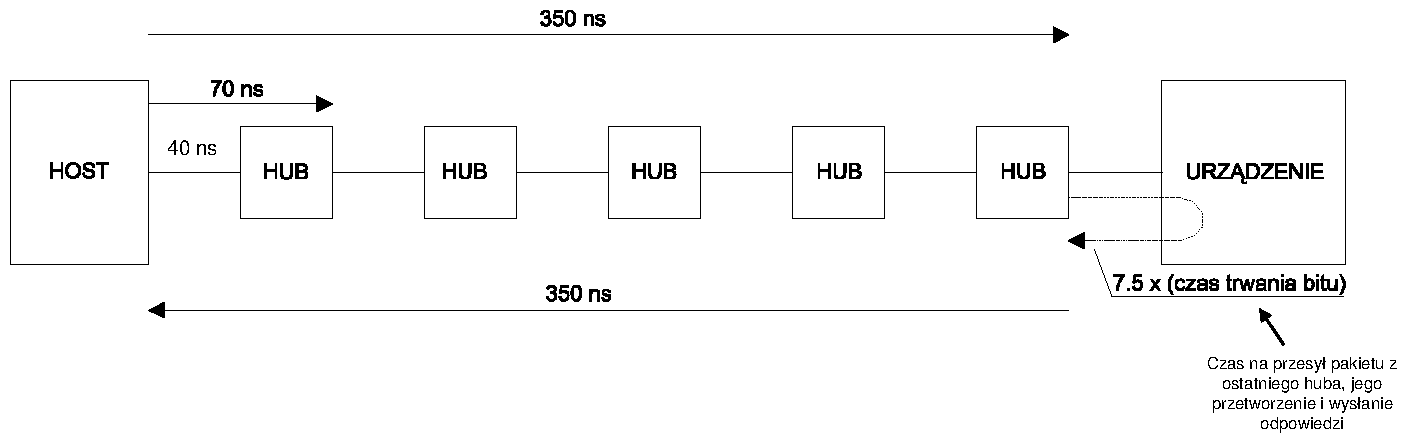
\includegraphics[width=10cm]{./wyklady/USB_23_1.pdf}
	\begin{itemize}
		\item Round trip delay: 2 x 350 ns = 700 ns
		\item Czas trwania 1 bitu full speed: 1/12 MHz = 83 ns
		\item Round trip delay w bitach dla full speed: 700 ns/83 ns = 8,5 bitu
		\item Timeout oczekiwania na odpowiedź: 7,5 bitu + 8,5 bitu = 16 bitów
	\end{itemize}
	
\subsection{Deskryptory w urządzeniach USB}
	\subsubsection{Hierarchiczna struktura deskryptorów w urządzeniu USB}
	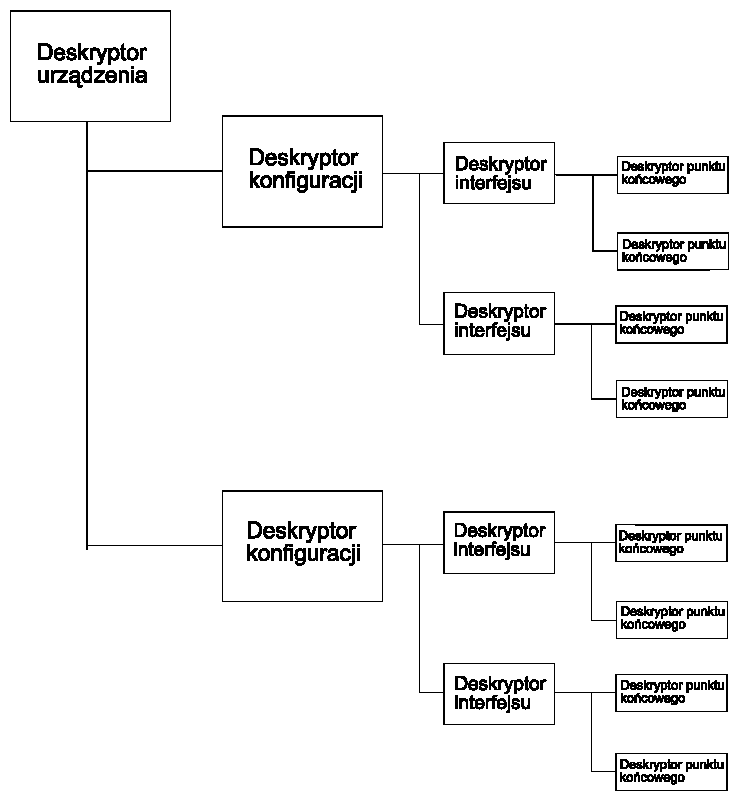
\includegraphics[width=10cm]{./wyklady/USB_24_1.pdf}
	\subsubsection{Rodzaje deskryptorów}
	\begin{itemize}
		\item Deskryptor urządzenia
		\item Deskryptor konfiguracji
		\item Deskryptor interfejsu
		\item Deskryptor punktu końcowego
		\item Deskryptor łańcuchowy
	\end{itemize}
	
\subsection{Wykrywanie i konfiguracja urządzeń}
	\subsubsection{Procedura enumeracji urządzenia}
	\begin{enumerate}
		\item Automatyczne wykrycie urządzenia
		\item Odblokowanie portu i generacja RESETU
		\item Odczyt deskryptora urządzenia
		\item Przypisanie adresu
		\item Odczyt pozostałych deskryptorów
		\item Konfiguracja urządzenia
		\item Instalacja sterownika klienta
		\item Urządzenie jest dostępne dla aplikacji
	\end{enumerate}
	
\subsection{Kontrola urządzenia – transfer kontrolny}
	\subsubsection{Etapy transferu kontrolnego}
	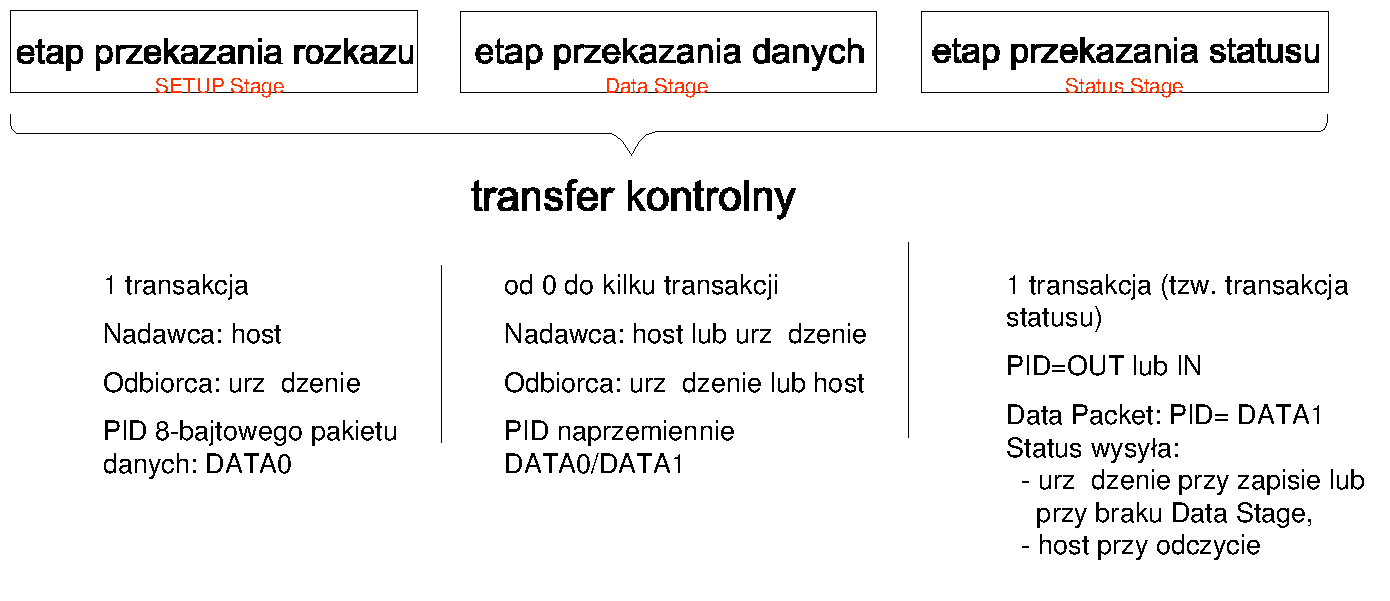
\includegraphics[width=10cm]{./wyklady/USB_31_1.pdf}
	
\subsection{Hub USB}
	\subsubsection{Co to jest?}
	Standard USB definiuje oddzielną klasę urządzeń: klasa HUB.
	\subsubsection{HUB zasilany z magistarli}
	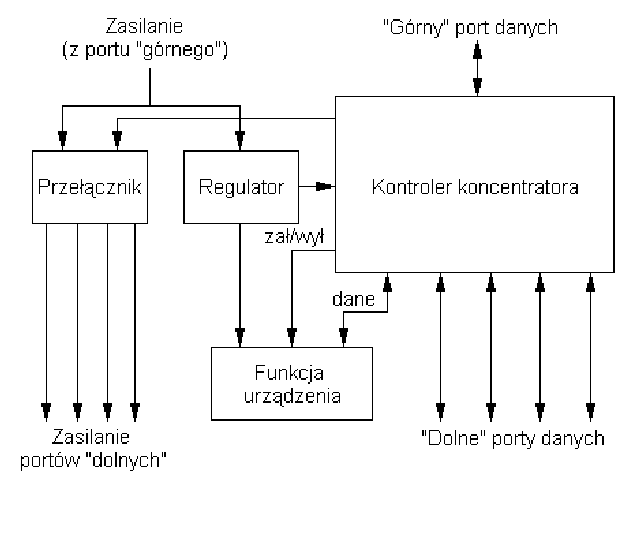
\includegraphics[width=10cm]{./wyklady/USB_34_1.pdf}
	\subsubsection{Proces konfiguracyjny huba}
	\begin{itemize}
		\item Odczyt standardowych deskryptorów urządzenia
		\item Przypisanie hubowi adresu
		\item Załączenie zasilania na porty, co jest niezbędne do detekcji podłączonych do portu urządzeń
		\item Odczyt punktu końcowego, "zmiany w hubie", w celu wykrycia urządzeń podłączonych do portów
		\item Odblokowanie portu w celu umożliwienia dostępu do urządzenia
	\end{itemize}
	\subsubsection{Punkt końcowy huba}
	\begin{itemize}
		\item \emph{Hub change point}: informuje o wystąpieniu:
		\begin{itemize}
			\item Zmiany w zasilaniu lub nadmiernym obciążeniu prądowym huba
			\item Zmiany na jednym lub kilku portach dolnych spowodowanej dołączeniem lub odłączeniem urządzenia.
		\end{itemize}
		\item Odczyt \emph{Hub change point} zwraca bajt statusowy huba
	\end{itemize}
	\subsubsection{Działanie}
	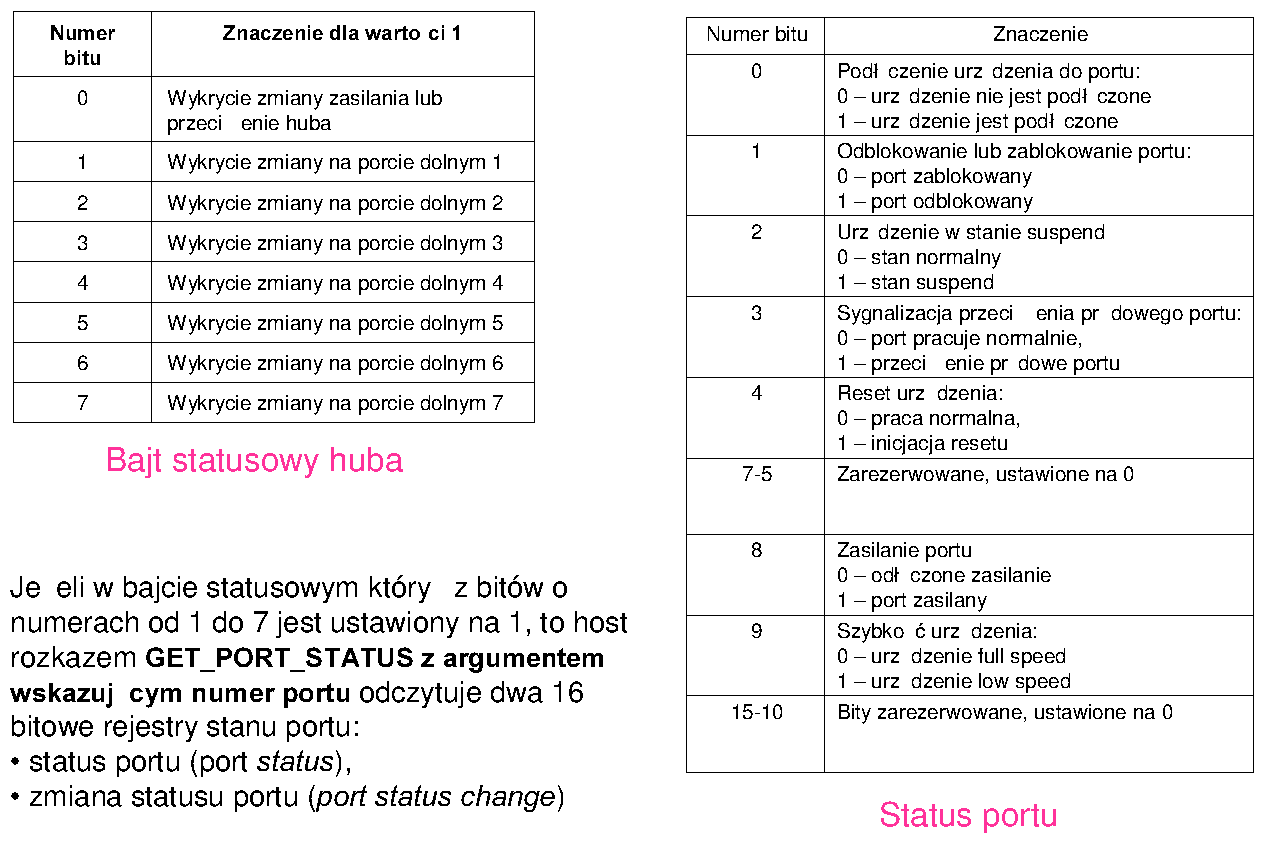
\includegraphics[width=8cm]{./wyklady/USB_35_1.pdf}
	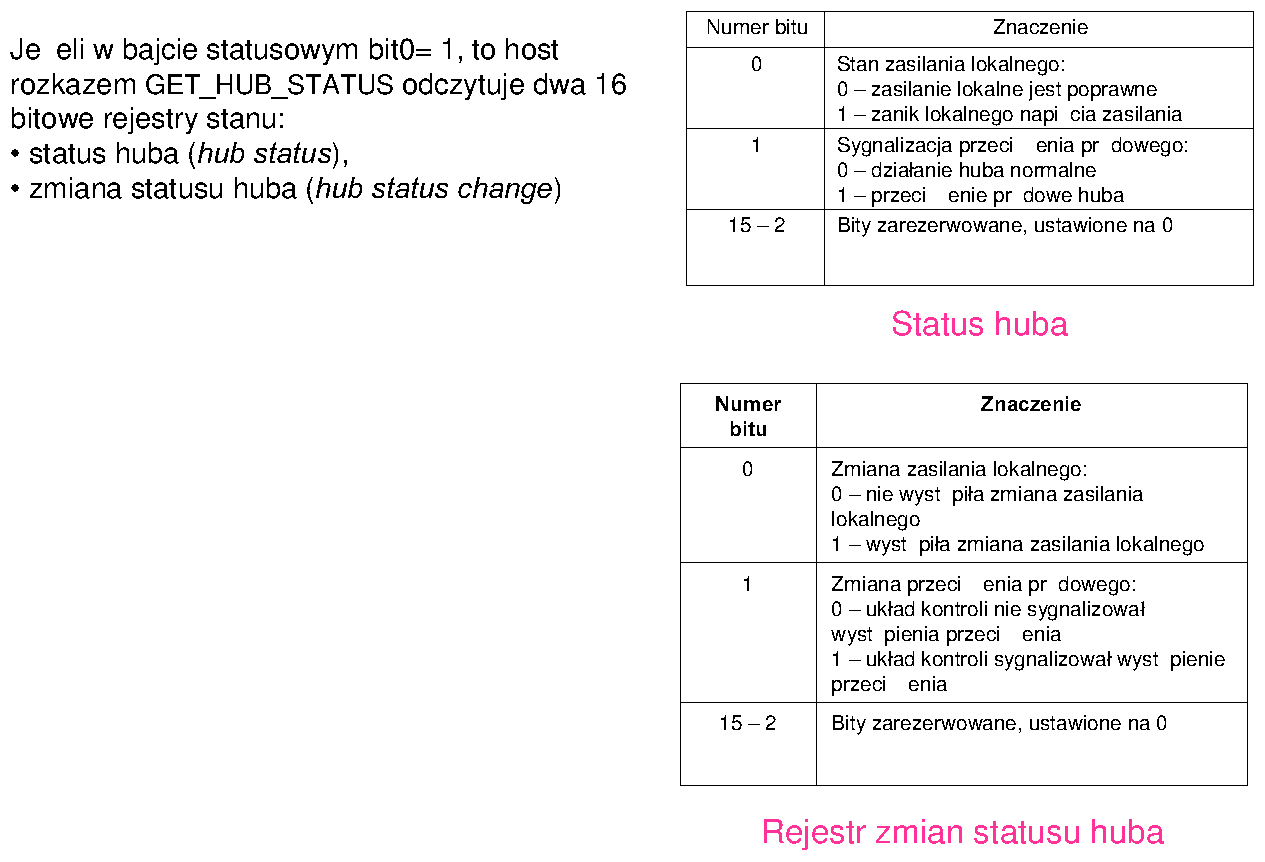
\includegraphics[width=8cm]{./wyklady/USB_36_1.pdf}
	
\subsection{Zasilanie urządzeń w systemie USB}
	\subsubsection{Rodzaje zasilania urządzeń USB}
	\begin{itemize}
		\item Urządzenie zasilane z magistrali
		\item Urządzenie zasilane z własnego źródła
		\item Urządzenie zasilane częściowo z magistrali i własnego źródła
	\end{itemize}
	\subsubsection{Zasilanie hubów i pozostałych urządzeń}
		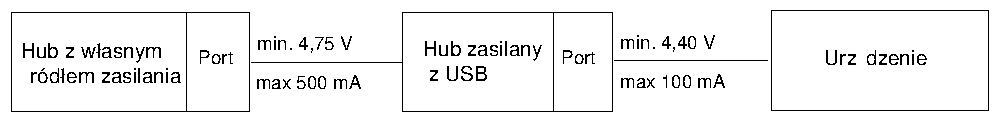
\includegraphics[width=11cm]{./wyklady/USB_38_1.pdf}\\
		Dopuszczalne spadki napięcia zasilania.
	\subsubsection{Urządzenie zasilane z magistrali}
		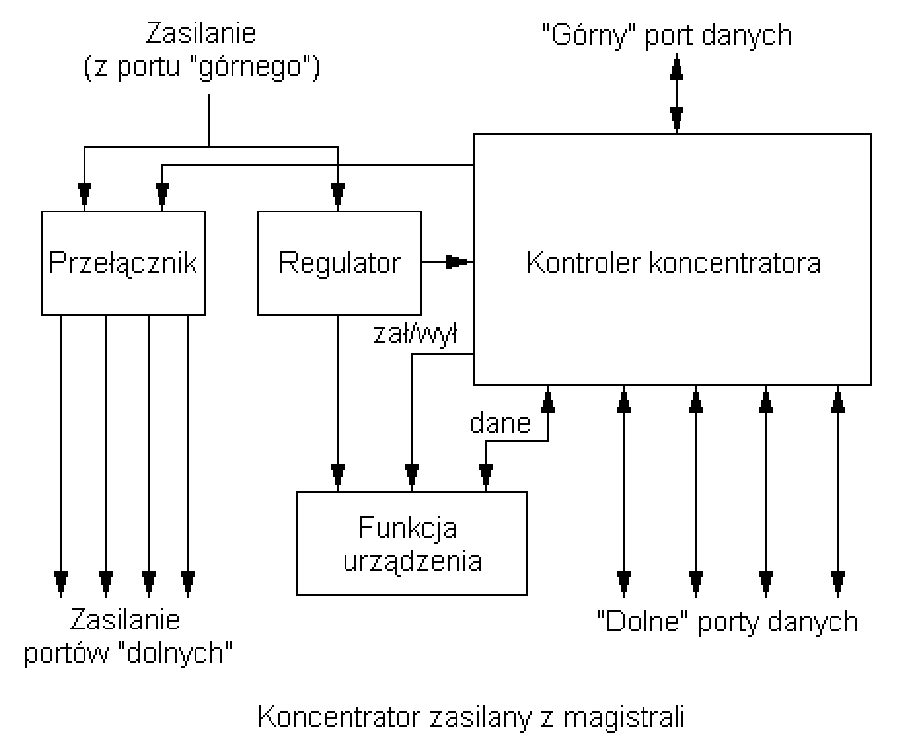
\includegraphics[width=7cm]{./wyklady/USB_39_1.pdf}
	\subsubsection{Zarządzanie zasilaniem}
	\begin{itemize}
		\item Zawieszenie pracy systemu – \emph{SUSPEND}
		\begin{itemize}
			\item \textbf{Globalne} - rozkaz SetPortFeature (PORT\_SUSPEND) adresowany do huba głównego
			\item \textbf{Częściowe} - rozkaz SetPortFeature (PORT\_SUSPEND) adresowany do huba zewnętrznego, w którym wybrany port ma zostać zawieszony.
			\item Zawieszone porty nie propaguj ruchu „w dół” oraz nie przekazuj „w gór ” żadnych sygnałów od urządzeń do nich podłączonych.
			\item Urządzenia w stanie zawieszenia zachowuj swój stan, co umożliwia wznowienie ich pracy bez ponownej konfiguracji.
			\item Hub w stanie zawieszenia dodatkowo blokuje wszystkie nadajniki, zatrzymuje wewnętrzne zegary i zachowuje stan wszystkich portów dolnych.
		\end{itemize}
		\item Wznowienie pracy systemu - \emph{RESUME} - po zawieszeniu
		\begin{itemize}
			\item Globalne
			\item Wake-up
			\item Wznowienie pracy urządzenia można nastąpić
			\begin{itemize}
				\item Z inicjatywy kontrolera, jako wznowienie po zawieszeniu globalnym lub częściowym\\
				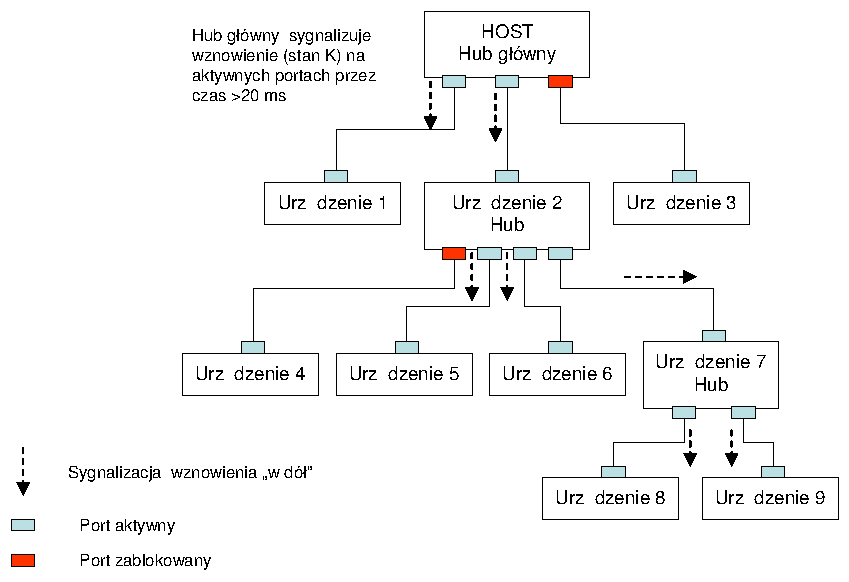
\includegraphics[width=7cm]{./wyklady/USB_43_1.pdf}
				\item Z inicjatywy urządzenia, po wystąpieniu zdarzenia wymagającego obsługi („budzenie” - \emph{Wakeup})\\
				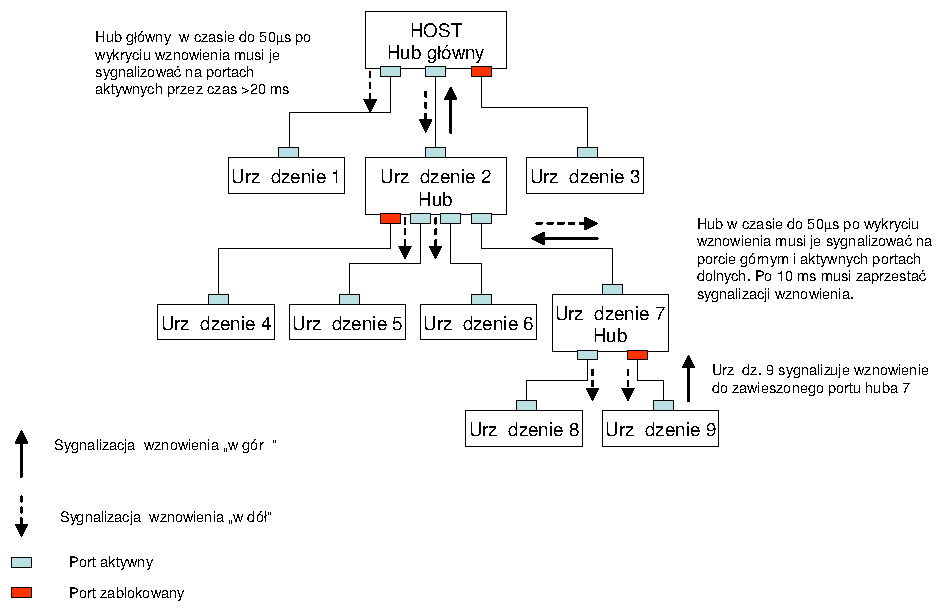
\includegraphics[width=7cm]{./wyklady/USB_44_1.pdf}
			\end{itemize}
			\item Wznowienie po zawieszeniu globalnym - rozpoczyna hub główny wykonując rozkaz wznowienia pracy systemu
			\item Wznowienie po częściowym zawieszeniu - może wykonać:
			\begin{itemize}
				\item Host rozkazem \emph{ClearPortFeature} (PORT SUSPEND) adresowanym do huba w którym znajduje się zawieszony port
				\item Urządzenie podłączone do zawieszonego portu poprzez \emph{Wakeup}
			\end{itemize}
		\end{itemize}
		\item Urządzenie pełnej szybkości (\emph{full speed}) automatycznie przechodzi do stanu \emph{SUSPEND} po wykryciu braku aktywności magistrali przez 3 $ms$.
		\item Urządzenie w stanie zawieszenie pobiera prąd $< 500 [\mu A]$
	\end{itemize}
\subsection{Rozwiązania host kontrolerów}
	\subsubsection{Co to jest?}
	Opracowano dwa rozwiązania host kontrolera:
	\begin{itemize}
		\item Uniwersalny host kontroler - \emph{Universal Host Controler} (Intel)
		\item Otwarty host kontroler – \emph{Open Host Controler} (Compaq, Microsoft, National Semiconductor)
	\end{itemize}
	\subsubsection{Uniwersalny host kontroler (UHC)}
	\textbf{Zasada działania kontrolera UHC}\\
	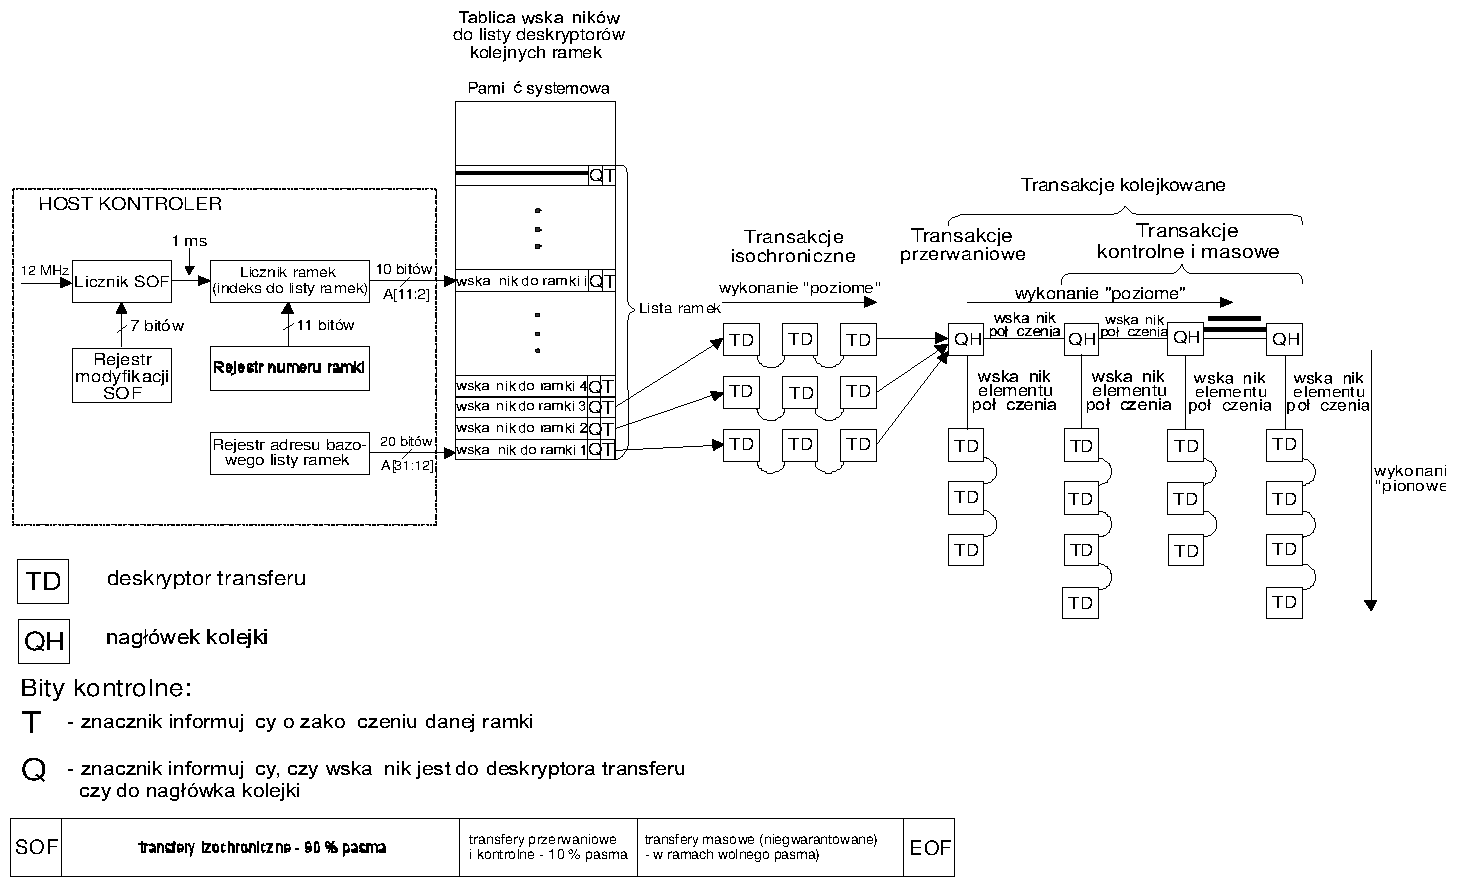
\includegraphics[width=7cm]{./wyklady/USB_46_1.pdf}\\\\
	\textbf{Ogólna postać deskryptora transferu (TD)}\\
	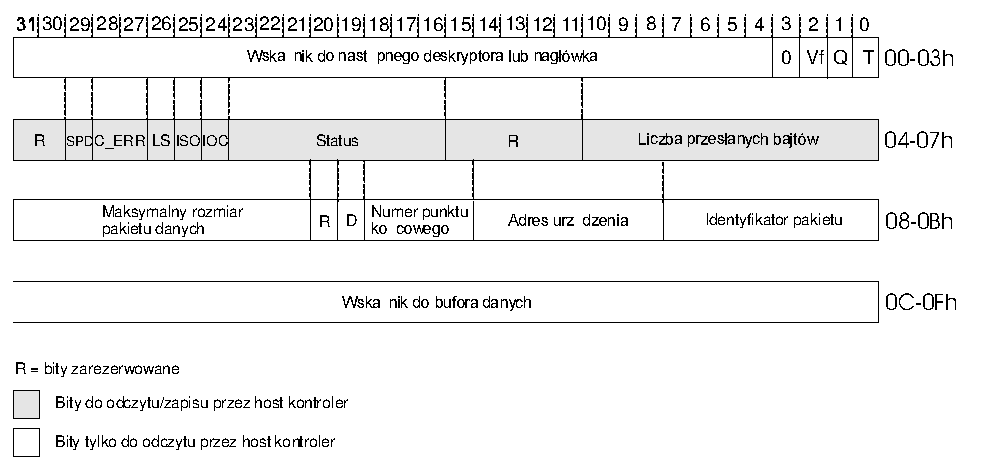
\includegraphics[width=7cm]{./wyklady/USB_47_1.pdf}\\\\
	\textbf{Ogólna postać nagłówka kolejki (QH)}\\
	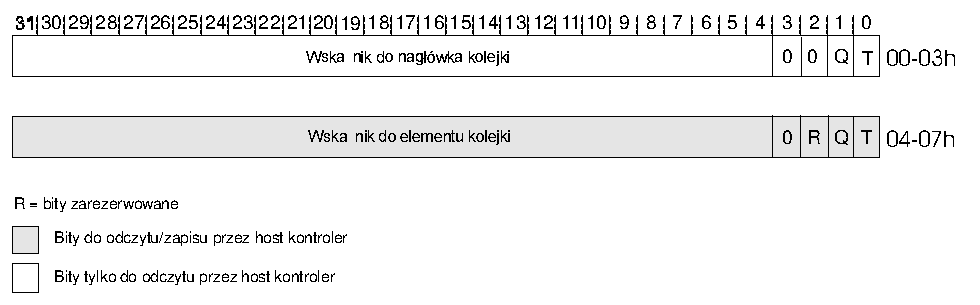
\includegraphics[width=7cm]{./wyklady/USB_48_1.pdf}
	\subsubsection{Otwarty host kontroler (OHC)}
	\textbf{Zasada działania kontrolera OHC}\\
	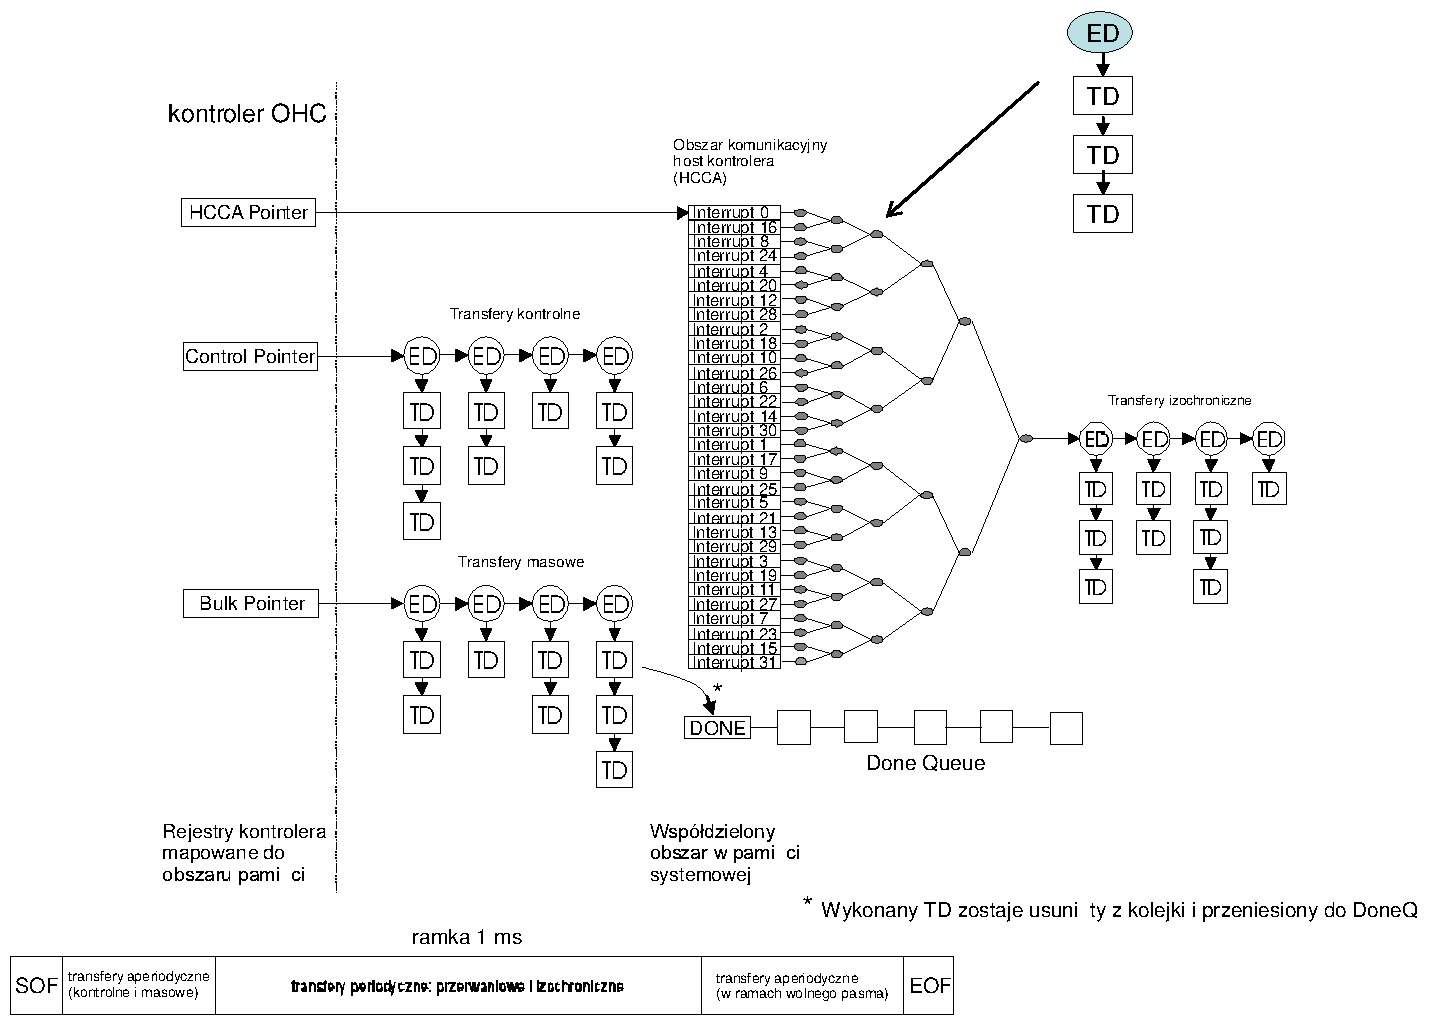
\includegraphics[width=7cm]{./wyklady/USB_49_1.pdf}\\\\
	\textbf{Format deskryptora punktu końcowego (ED)}\\
	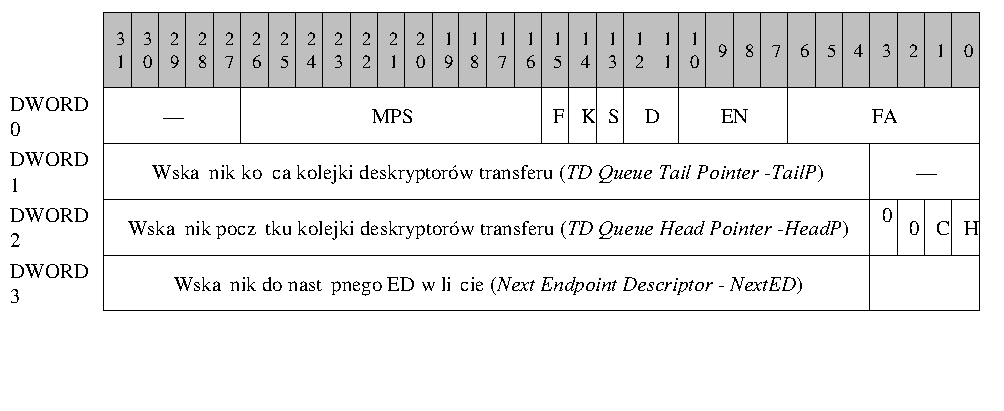
\includegraphics[width=7cm]{./wyklady/USB_50_1.pdf}\\\\
	\textbf{Ogólna postać deskryptora transferu (TD)}\\
	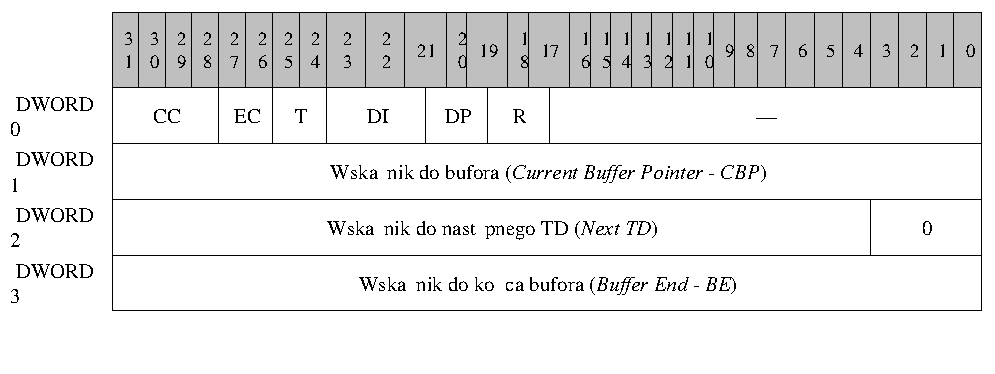
\includegraphics[width=7cm]{./wyklady/USB_51_1.pdf}
	
\subsection{USB 2.0 - rozszerzenie standardu}
	\subsubsection{Ważniejsze elementy wprowadzone w USB 2.0}
	\begin{itemize}
		\item Wysoka szybkość transmisji (high speed) - 480 Mb/s
		\item Protokół PING-NYET
		\item Transakcja SPLIT
		\item Komunikacja z szerokopasmowym punktem izochronicznym
		\item Nowe typy pakietów
	\end{itemize}
	\subsubsection{Wysoka szybkość transmisji}
	Podział ramki na 8 mikroramek wysokiej szybkości\\
	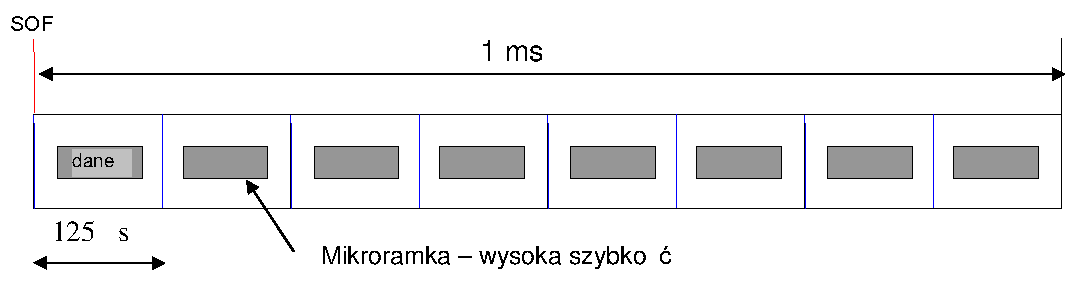
\includegraphics[width=7cm]{./wyklady/USB_53_1.pdf}
	\begin{itemize}
		\item Mikroramka trwa 125 $\mu s$
		\item Na 1 ramkę przypada 8 mikroramek
		\item Wysoka szybkość transmisji - w mikroramce wynosi 480 Mhz.
	\end{itemize}
	\subsubsection{Protokół PING-NYET}
	Potwierdzenie NYET (\emph{NOT YET}) dla urządzeń \emph{high speed}.\\
	\textbf{Problem:} przy zapisie do urządzenia, jeżeli nie jest ono „gotowe na dane” potwierdzenie negatywne przychodzi dopiero po pakiecie danych – strata czasu.\\
	\textbf{Rozwiązanie}:\\
	TOKEN PING – zapytanie urządzenia, czy jest gotowe do przyjścia danych.\\
	Możliwe odpowiedzi i reakcja hosta:
	\begin{itemize}
		\item ACK – wykonanie transakcji OUT
		\item NYRT – host kontynuuje wysyłanie zapyta PING
	\end{itemize}
	\textbf{Korzyści}: lepsze wykorzystanie magistrali (PING jest krótki).
	\subsubsection{Transakcja SPLIT}
	\textbf{Problem:} Host i hub wysokiej szybkości komunikują się z urządzeniem małej lub pełnej szybkości. Szybkie przesyłanie danych pomiędzy hostem i hubem oraz wolne pomiędzy hubem i urządzeniem – konieczność buforowania danych w hubie.\\
	\textbf{Rozwiązanie}:\\
	Transakcja dzielona, złożona z dwóch części:
	\begin{itemize}
		\item SSPLIT (\emph{Start Split} - rozpoczęcie transakcji dzielonej)
		\item CSPLIT (\emph{Complete Split} – zakończenie transakcji dzielonej).
	\end{itemize}
	\subsubsection{Komunikacja z szerokopasmowym punktem izochronicznym}
	Komunikacja z „normalnym” izochronicznym punktem końcowym zakłada jedną transakcję na ramę lub mikroramkę.\\
	W przypadku punktów szerokopasmowych, obsługiwanych tylko przez kanały \emph{high speed}, istnieje możliwość przekazania w jednej mikroramce większej ilości danych wykonując bezpośrednio po sobie od jednej do trzech transakcji.\\
	Dane w takiej sekwencji transakcji muszą być oznaczone, przy czym nie wystarczą już „znaczniki” Data 0 i Data 1, dlatego wprowadzono dwa kolejne typy pakietów danych: \textbf{Data 2} i \textbf{MData}.\\
	Pakiet \textbf{Data 2} wykorzystywany jest przy odczycie danych z urządzenia, natomiast \textbf{MData} i \textbf{Data 2} przy zapisie do urządzenia.\\
	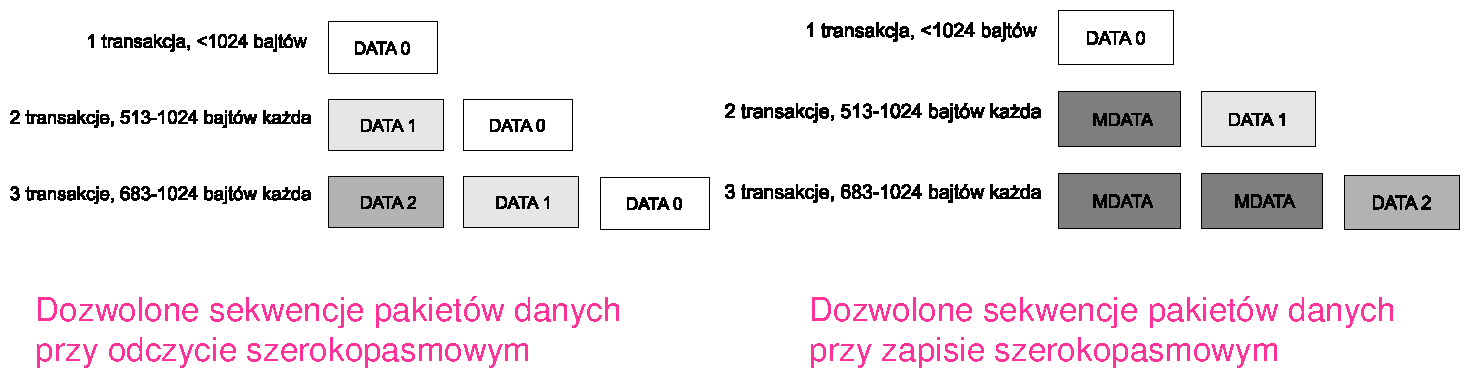
\includegraphics[width=15cm]{./wyklady/USB_56_1.pdf}
	\subsubsection{Specjalne pakiety TOKEN wprowadzone w USB 2.0}
	Kody pakietów specjalnych zgodnie z USB 2.0\\
	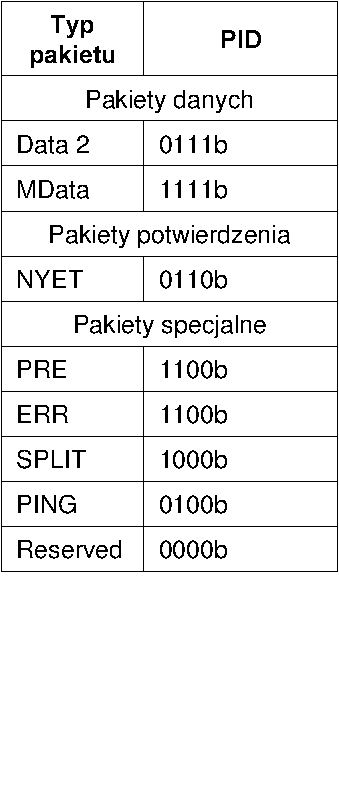
\includegraphics[width=3cm]{./wyklady/USB_57_1.pdf}
	
\section{IEEE-488 and SCPI standards}
\section{IEEE-1394 (FireWire)}
\section{Tłumienie zakłóceń w rozproszonych systemach komputerowych}
\end{document}